\documentclass[12pt]{article}

% Packages
\usepackage{fullpage}
\usepackage{graphicx}
\usepackage{caption}
\usepackage{array}
\usepackage{tabularx}
\usepackage{cleveref}
\usepackage[figuresleft]{rotating}
\usepackage[citestyle=reading,backend=bibtex]{biblatex}
\newcolumntype{L}[1]{>{\raggedright\let\newline\\\arraybackslash\hspace{0pt}}m{#1}}
\newcolumntype{R}[1]{>{\raggedright\let\newline\\\arraybackslash\hspace{0pt}}m{#1}}



% Biblatex setup
\addbibresource{bibliography.bib}

% Commands
\newcommand{\HRule}{\rule{\linewidth}{0.5mm}}

% Setup
\author{Team Hydra}
\title{Final Report}

% Doc structure
\begin{document}

  \begin{titlepage}
\begin{center}


\includegraphics[width=0.08\textwidth]{./img/lu-logo.png}~\\[3cm]

\textsc{\LARGE Loughborough University}\\[2.5cm]

\textsc{\Large Group Project}\\[0.5cm]

% Title
\HRule \\[0.4cm]
{ \huge \bfseries Final Report \\[0.4cm] }

\HRule \\[1.5cm]

% Authors
\noindent
\large
\emph{Team Hydra:}\\
Jay \textsc{Vagharia}\\
Oliver \textsc{Woodings}\\
Simon \textsc{Kerr}
\vfill

% Bottom of the page
{\large May 2015}

\end{center}
\end{titlepage}
  \tableofcontents
  \clearpage
  \section{Introduction}

\subsection{Background}
As part of this module, we were entered into an International IT Challenge run by \emph{Atos}.  Amos publicise this competition to many universities where students will attempt to create a solution to the requirements set by Atos.  This year the challenge revolved around \emph{Connected Living}.  There are many definitions for connected living.  Some definitions define it as something constrained to the home.  Others describe it as a world where customers use different devices to experience connection anytime, anywhere.  This definition covers connected homes, connected work and connected city.  Atos believe that connected living involves bringing the home, workspace and city seamlessly together through smart devices providing connectivity anytime, anywhere.  Consumers are always wanting to feel more connected to their workspace, their homes and their cities.  \\
Originally, there were a few objectives set by Atos that they wished to be fulfilled:
\begin{itemize}
\item Easy Connection of Products
\item Big Data Analytics
\item Create an Audience
\item Client Facing App
\end{itemize}
We tried to think outside the box for this project and decided not to create an app that would deal with the ``connected home'' but something that has never been created before and something we feel still meets the criteria laid out by Atos.  As a team, we wanted to create something that would enhance peoples social lives and provide a service both to the customers and the businesses involved.  

\subsection{The Customer}
From Atos, we are assigned a mentor who acts as a customer.  We have been allocated \textbf{Mike Smith}; a Chief Technology Officer within Atos.  Mike has extensive knowledge of all things technical and has recently written a paper about \emph{Connected Train}.  This makes him an ideal customer as he has knowledge of the \emph{Connected World}.  We aim to tap into this knowledge and gain advice and feedback in order to improve and enhance our idea from its born until the end of this module.  

\subsection{The Team}
Team \textbf{Hydra} involves three Computer Science Masters students; Jay, Oliver and Simon. Being computer scientists, we have a high interest in technology (with a small geek streak) with a passion for music.  We have all successfully completed an industrial placement, which provides us with the necessary skills to complete this project.  We have briefly defined our roles as follows based on our strengths and weaknesses.  

\begin{center}
  \begin{table}[h]
  \begin{tabular}{|l|l|l|}
  \hline
  \multicolumn{1}{|c|}{\textbf{Name}} & \multicolumn{1}{c|}{\textbf{Role}} & \multicolumn{1}{c|}{\textbf{Responsibilities}}                                                                                                                                      \\ \hline
  Jay                                 & Project Secetary, Client Side Developer         & \begin{tabular}[c]{@{}l@{}}Organising meetings and following \\* the project timeline.\\ Assisting with development where \\* possible.\end{tabular} \\ \hline
  Oliver                              & Project Manager, Technical Lead                     & \begin{tabular}[c]{@{}l@{}}Leading the technical aspects of the \\* projects forward.\\ Managing cloud infrastructure for \\* both documentation and code.\end{tabular}                     \\ \hline
  Simon                               & Business Development, Client Side Developer    & \begin{tabular}[c]{@{}l@{}}Carrying the app forward according \\* to the business model in terms \\* of legal and technological factors.  \\ UI development\end{tabular}                                                              \\ \hline
  \end{tabular}
  \end{table}
\end{center}

\subsection{The Idea}
In order to create something new, we steered away from the connected home.  We wanted something different, something unique and that took us towards music.  So we started off with trying to connect people with music.  We want to provide the ability to connect to and control the music in your surroundings, anywhere.  We want users to walk in to a coffee shop, library, bar, restaurant etc. and have the ability to suggest their favourite songs that are then played through the public audio media.  \textbf{Choona} is an app focused around the `Connected Music'.  Our research has shown there is no music sharing concept that allows people to collaboratively listen, interact and suggest music to people in your surrounding area, home or business through an intelligent, cloud-driven playlist system.  \\
Choona is a public music player that lets you have a say in what you listen to in public, allowing you to suggest songs that you want to be played at your location.  It provides you with the option to like/dislike songs suggested by others, where increased likes on a song will push that song further up the order allowing it to be played sooner.  Furthermore, you can connect through your mobile device allowing you to listen to the music privately (via your headphones).  \\
Choose provides many different features for the businesses involved.  Advertisements can be added in two forms; visual or audio thus improving product/promotional awareness.  Furthermore, it gives the customer the opportunity of selecting what they want to hear thus keeping them happy.  The 
  \clearpage
  \section{Project Plan}

\begin{minipage}{\linewidth}
  \hspace*{1.7in}
  \begin{rotate}{270}
    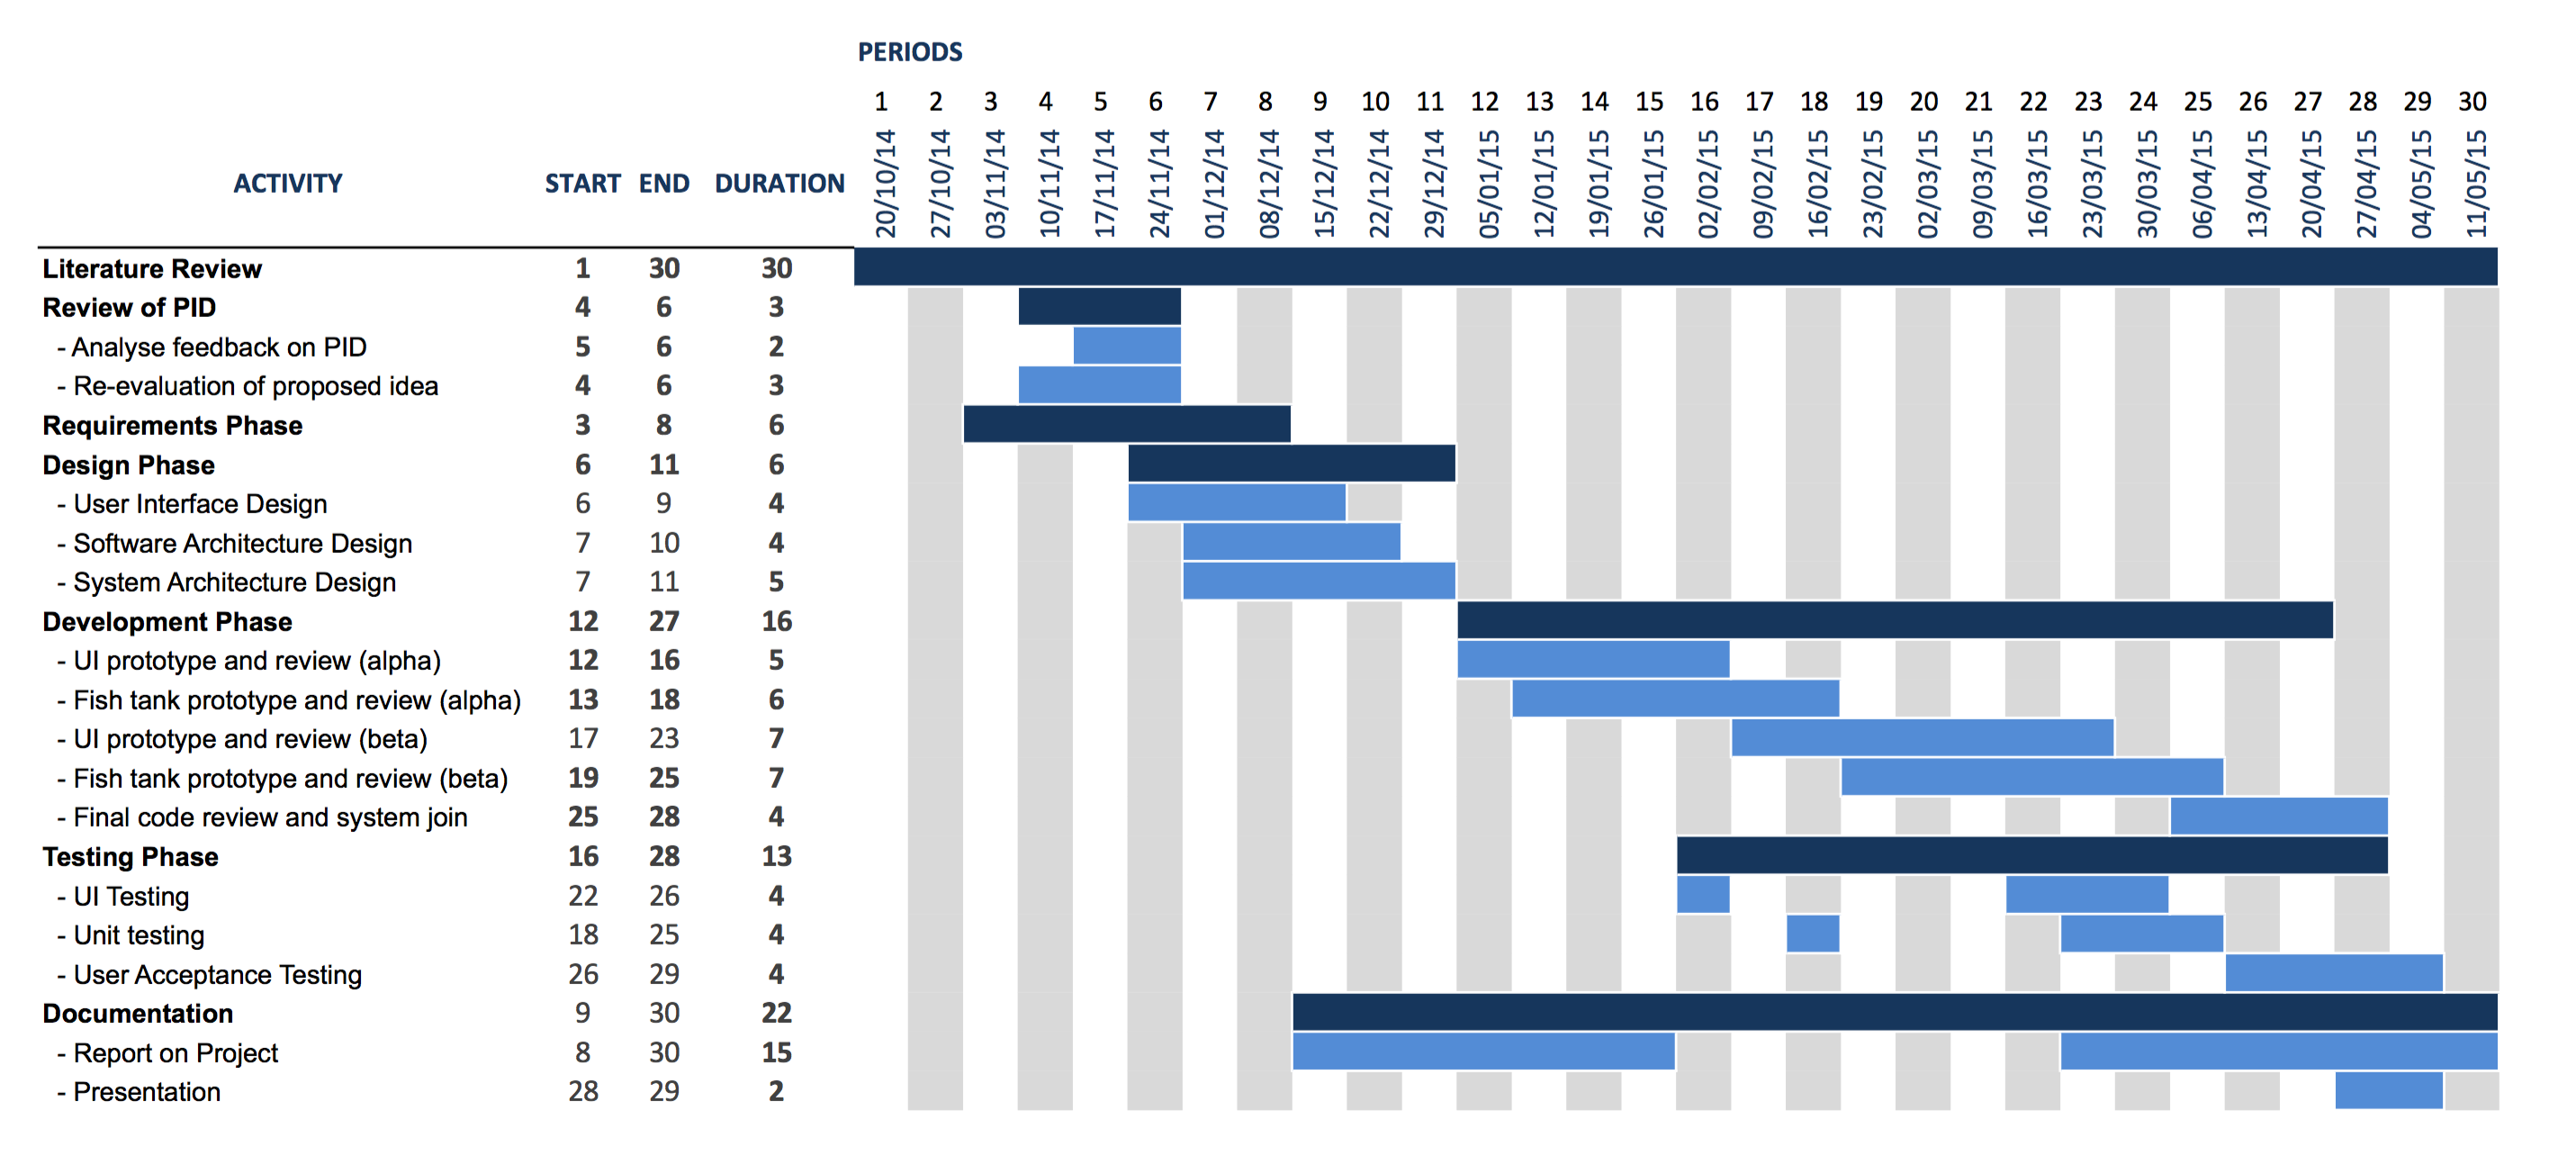
\includegraphics[width=1.28\textwidth]{./img/gantt_chart.png}
    \label{gantt_chart}
  \end{rotate}
\end{minipage}
\clearpage

\subsection{Gantt Chart}
The gantt chart we have provided illustrates how we will aim to complete this project on time.  It includes a break up of all the tasks and the proposed start and finish times.  We will use this gantt chart to track our progress throughout the project and there may be cases whenever we have had to adjust it due to time constrains and other activities outside the project.  \\

\textbf{Milestones} are tasks with zero duration.  This is because they highlight an important achievement in the project and therefore by the time this milestone has been reached, a specific part of the project should be completed.  We have used the red diamond icon to signify a milestone in the gantt chart.  \\
Meetings with the client have been identified as milestones as substantial progress needs to have be shown to the client each time we meet them.  Other milestones include the a complete working prototype and a finished documentation.

\subsection{Phases and Deliverables}
This project will entail a number of different deliverables positioned around the different phases.  In the below table, we have ordered the phases and deliverables chronologically.  Each deliverable will be reliant on the completion of the previous phase(s).  We can use these dates to track our progress.  Keeping track of progress will allow us to access our position and determine whether or not we are on schedule to complete the project on time.  If this is not the case, we will have realised in time to make the necessary adjustments that will result in us meeting the completion date of the whole project.  \\

\noindent
\begin{tabular}{|l || p{6cm}|}
\hline
\textbf{Phase/\emph{Deliverable}} & \textbf{Date Due} \\ \hline
Review of PID & 24/11/2014 \\ \hline
\emph{Client meeting for requirement analysis} & 26/11/2014 \\ \hline
Requirements phase & 12/12/2014 \\ \hline
Design Phase & 04/01/2015 \\ \hline
\emph{Client meeting for UI analysis} & 16/04/2015 \\ \hline
Development Phase & 27/04/2015 \\ \hline
Testing phase & 04/05/2015 \\ \hline
\emph{Demonstration of prototype} & 16/04/2015 \\ \hline
Completion of project and Documentation hand-in & 14/05/2015 \\ \hline
\end{tabular}\\
\vspace{0.5cm}

\subsection{Team Roles}
We have tried to arrange the team according to our strengths and weaknesses.  We have tried to consider the different tasks involved in the project and identify the roles that an individual is most likely suited to.  \\
According to Belbin, there are 9 different team roles; three action roles, three people roles and three thought roles.  Our team cover the majority of roles between them; we have shapers, implementers, completes, plants specialists, monitor and team-workers.  Overall this provides us with problems solvers and passionate specialists that have a wealth of knowledge as well as individuals that have a  motivation to complete this task on time and to a high standard. \\
Below, we have defined our roles within the team to best suit our skills and to suit the type of role we are stronger at.

\begin{center}
  \begin{table}[h]
  \begin{tabular}{|l|l|l|}
  \hline
  \multicolumn{1}{|c|}{\textbf{Name}} & \multicolumn{1}{c|}{\textbf{Role}} & \multicolumn{1}{c|}{\textbf{Responsibilities}}                                                                                                                                      \\ \hline
  Jay                                 & Project Secetary, App UI        & \begin{tabular}[c]{@{}l@{}}Organising meetings and following \\* the project timeline.\\ Assisting with development where \\* possible.\end{tabular} \\ \hline
  Oliver                              & Project Manager, Technical Lead                     & \begin{tabular}[c]{@{}l@{}}Leading the technical aspects of the \\* projects forward.\\ Managing cloud infrastructure for \\* both documentation and code.\end{tabular}                     \\ \hline
  Simon                               & Business Development, App UI    & \begin{tabular}[c]{@{}l@{}}Carrying the app forward according \\* to the business model in terms \\* of legal and technological factors.  \\ UI development\end{tabular}                                                              \\ \hline
  \end{tabular}
  \end{table}
\end{center}

\subsection{Project Management}

Responsibilities will be shared throughout the project as there are only three people in the team.  The roles will change throughout the project as it may suit someone else to take on a responsibility at certain stages.  There will also be times when experience will become a factor; we have considered this and tried to align our team roles to match.  During different stages of the project, it may be that we have different activities going on outside of the project that may cause slight readjustments to the gantt chart but this will not effect the overall outcome.  The stronger programmer(s) in the team will have a better understanding of what is involved at the development stage of the project therefore they will be more inclined to take responsibility and delegate tasks.  \\
Every week, we will meet up to discuss any feedback we have based on our previous weeks work and if any decisions need to be taken based on this, these will be made clear and a decision taken before the meeting finishes.  If a decision cannot be taken because of lack of information, we will go away and research the area further and bring the relevant issue(s) up at the next meeting.  We will also use these meetings to determine whether or not we are currently on schedule with the project and to make proactive decisions based upon our current rate of progress.  During each meeting, we will decide what each members tasks for the next week thus allowing us to allocate the right amount of time to complete them.

\subsubsection{Team Communication}
The main communication method for all team members will be through a ``WhatsApp'' group.  All member currently use this as a social messaging service therefore we felt it was a good idea to use this as we always have access to it.  The main idea of this is to send short messages to each other whether it be the whole group or just one individual.  This keeps everyone in the loop.  We can effectively use this to organise meetings and communicate our progress and problems.  We also have gmail accounts that allow us to send communications to our customer (Mike).  \\

Further to this, we all have access to ``Google Drive''.  We have used this to create a folder that each of us have access to.  Here we can post any documents we want the other team members to view and they can instantly access them and make any changes they want; these changes will be globally updated for all users to see.  \\
Initially a ``Trello'' discussion board was used to throw ideas around and discuss potential features of the app as well as a broad business model. \\
We will also be using GitHub.  GitHub is a web based repository that offers Source Code Management (SCM).  SCM is a necessity in a team orientated software development project.  A Version Control System (VCS) allows the developers to make revisions to the code seamlessly and without overwriting someone else changes.  It also allows you to revert to previous versions or examine them where need be; to help identify issues with newer version(s).  This is a very useful tool to have especially when the project involves such a large code base and multiple developers.  

\subsection{Resources}
In order to complete this project, there will be several different resources we will need to have access to.  This can usually be split into three different categories; personnel, funds and non-personnel.  However for this project, the only personnel we have are the three team members and this cannot be expanded on.  Funds is also non-negotiable; standing at £0.  \\
We do have several non-personnel resources - these are resources that we need in order to produce the prototype and documentation.  These are listed below with an explanation as to why these are needed.
\begin{itemize}
\item Raspberry Pi - There is the potential for some software to be developed and put on a hardware device in order to connect with the cloud and stream audio (music).  For prototyping it is likely that pre-existing devices such as the Raspberry Pi will be used. 
\item Speakers - To enable us to listen to the output from the Raspberry Pi
\item Laptops - these enable us to work as a team in any location at any time and for use in the presentation.  
\item Television - to present our idea and prototype at the end of the year.
\end{itemize}
Having the above items will make sure we can complete this project to a good standard and bale us t give a presentation at the end.    

\subsection{Software Development Approach}
Software Development Approaches have existed since the 1970s. They range from rigid, long-term methods such as \emph{Waterfall}. through to experimental and risky approaches like \emph{Extreme Programming}. Factors such as team size, business goals and clients all contribute to choosing the correct approach.\\
To identify the correct software development process to use we must first decide on some attributes of the project of which we can compare across various approaches. The following have been derived from the project ideas and plan:

\begin{enumerate}
  \item \textbf{Team Size} -
    Most of the development throughout this project will be done by one person. This removes the need for large-scale approaches such as \emph{Waterfall} and \emph{Spiral} and instead opens up the possibility of a faster, looser process such as \emph{Agile}.
  \item \textbf{Client Interaction} - 
    If the project idea is accepted we will be allowed to work very closely with a representive from Atos. This means our development approach needs to incorporate this throughout the entire lifecycle, making methodologies such as \emph{Waterfall} less relevant since they do not encourage client interaction during the development stage.
  \item \textbf{Timeline} - 
    The entire development and testing cycle for the project is only a few months, so whatever approach is chosen needs to be dynamic and allow for quick iterations without the need to go through the entire process again. This requirement makes approaches such as \emph{Incremental Development} inappropriate because they add in repeated requirements analysis and architecture design steps that may not be necessary.
  \item \textbf{Deliverable} -
    The client is expecting a working prototype to be delivered at the end of the project. The technology must be built to a satisfactory standard, but does not need to be production-ready nor be immaculately written. This allows for the testing, integration and implementation steps in the software development approach to be removed as a priority and opens up the possibility of using less formal approaches such as \emph{Prototyping} and \emph{Extreme Programming}.
\end{enumerate}
These requirements narrow the scope down to three relevant approaches.  The first one is \textbf{Agile}.  Agile development promotes principles such as continuous improvement, early delivery, adaptive planning and evolutionary development. It breaks tasks down into small increments, with the goal of each increment being a new release. There is a big focus on quick communication and easy feedback, normally achieved by daily standup meetings and regular planning sessions. Whilst the communication principles would be useful for this project, the approach also tends to have a reliance on multiple teams tackling the project which is not relevant.\\
The second approach we could take would be \textbf{Prototyping}.  Software prototyping is perfect for projects where a production-ready deliverable is not required. Each iteration of the project has no requirement to fully work or meet the users' requirements. Instead, the software goes through an iterative modification process until user acceptance is met or the prototype is discarded.  The downfall of prototyping is that it is a very relaxed approach. Client interaction is suggested, not enforced, and often the developers may lose sight of the completed project by getting too involved in a limited prototype which ultimately is only a partial representation of the desired product.\\
Finally, we have \textbf{Rapid Application Development (RAD)}.  RAD is used to describe alternatives to the \emph{Waterfall} approach that focus on iterative development rather than formal, structured planning cycles. The most common definition of RAD, created by James Martin, involves an initial requirements planning stage followed by an iterative construction and user feedback stage.\\

    \begin{minipage}{\linewidth}
      \centering
      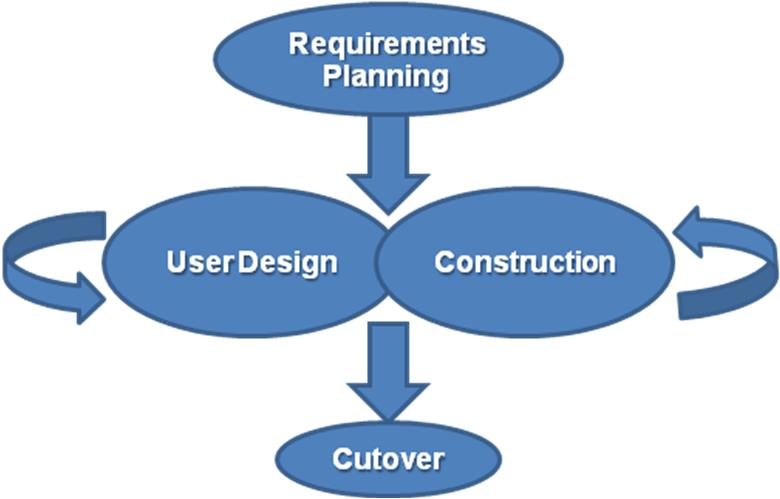
\includegraphics[width=0.5\textwidth]{./img/rad-model.jpg}
      \captionof{figure}{Phases in the James Martin approach to RAD}
    \end{minipage}\\

RAD fits in nicely with the four primary project attributes that we defined above.  RAD has no mandatory definition for team size or interactions.  It requires that development, client feedback and testing go hand in hand.  For this type of project this is ideal.  RAD does not stipulate a restriction on the length of the project thus allowing for the development cycle to be as long as possible before the deadline is reached without the need to stipulate iterations during the planning stages.  Finally, there are no requirements for repetitive testing and quality control.  This can be implemented independently from the software development approach, allowing for testing to be suited to the individual project.\\
The analysis above clearly identifies \textbf{Rapid Application Development} as the most appropriate software development approach for this project.

\subsection{Technical Considerations}
The technical considerations for this project can be divided into two sections: mobile application and server-side systems.

\subsubsection{Mobile Application}
One of the basic top-level requirements for this project is that the end product is centered around a mobile application.  Therefore it is important to ensure that all the technology used or idealised is compatible with as many mobile devices as possible.  If the app starts to have a dependency on niche features, such as NFC and 4G, there is a risk of excluding large quantities of users.\\
For a mobile application, we must consider the platform.  There are currently three major mobile platforms that support apps: Android, iOS and Windows Phone.  Others like Blackberry and Firefox OS either do not have a thriving application community or have a very small user-base.  This project should ideally support all three of the major platforms.  The problem with this is that each one requires applications to be written in different languages.  In order to come to a decision, we need to consider the following:
\begin{itemize}
\item \emph{Native Applications} - A native application is one that is written to work directly with the device's operating system. For example on Android this would mean that the application is written in the programming language Java and that it directly uses the device's native libraries. The advantage this approach is mainly performance, but there are also certain features that are only available for native applications. The disadvantage is that the application has to be written separately for each platform you want to support.
\item \emph{Framework Applications} - To solve the difficulties of supporting multiple platforms, frameworks such as Apache Cordova and Adobe Phonegap have been created. These allow developers to write their applications once and have it automatically work across all major platforms. The downside here is that the application normally exists inside a `wrapper' which can have a negative impact on performance.  \\
Phonegap allows users to develop hybrid mobile device application; an app that is neither a native mobile app (as layout rendering is done via web views instead of a platform native UI framework) nor a pure web-based app (because they are packaged as apps for distribution and have access to native device APIs).  At this point, we then need to make another decision; how we are going to build the web app?  There are two methods we can choose from; writing the whole app in pure JavaScript, HTML and CSS.  This requires a lot of effort thus most people will opt to use a regular framework e.g. AngularJS, ReactJS or EmberJS but there is one small issue with these frameworks; they are not specifically designed for mobile app development (`mobile-first').  Ideally if we want to create an app, we want to use a framework that is specifically designed to create them i.e. a framework that makes use of another framework.  One example is \textbf{Ionic}.  Ionic (making use of AngularJS) is a suite of components and styles that are mobile friendly hence making it perfect for app development.
\end{itemize}
The \textbf{Technology} behind the mobile device is another area of consideration.  Features such as NFC are starting to become prevalent in many high-end smartphones yet there are still devices that block the use of such technology (such as the iPhone range - the iPhone 6 does have NFC capability but this is only available for apple pay) and there are devices that don't have this capability purely because they are on the lower-end of the market. 

\subsubsection{Server-Side Systems}
Many ideas and concepts in this project revolve around connected data and technology. There are likely to be many different services and systems required in order to complete the project. Designing and architecting will be an important part of ensuring the project is a success.  \\
There are many different styles of \textbf{Software Architecture}. For this project we will be using the \emph{Microservices Architecture}. This is centered around separating out the application into individual services, each one with its own unique responsibility. This fits in nicely with the chosen Software Development Approach - \emph{Rapid Application Development} - since it allows for entire services to be completed in a single development cycle.\\

    \textbf{Advantages}
    \begin{itemize}
      \item Easier debugging
      \item Better fault isolation
      \item Independent service development and deployment
      \item Removes commitment to a specific technolog stack
      \item Avoids monolithic applications and systems
    \end{itemize}

    \textbf{Disadvantages}
    \begin{itemize}
      \item Requires inter-service communication
      \item Testing can be more complicated
      \item Multi-service deployment can be hard to orchestrate
      \item Multiple services means more memory usage
    \end{itemize}
A solid \textbf{Infrastructure} is essential in order to adequately support the numerous software services and systems required for the project. There are several options available when it comes to selecting infrastructure components (servers, database management systems etc):
    \begin{itemize}
      \item \textbf{Cloud Computing} - 
        Cloud-based systems such as \emph{Amazon Web Services} (AWS) and \emph{IBM SoftLayer} allow systems engineers to easily configure and deploy scalable services across the globe. They often support many different types of services (application servers, databases, data processors, queues etc) and can be configured quickly and easily through user interfaces, rather than having to manually set up each service. The downside to cloud-based infrastructure is usually the cost and also the added abstraction; the systems engineer is no longer in direct control of each moving part which can sometimes make fault finding a more laborious process.
      \item \textbf{Dedicated Servers} - 
        Dedicated servers are the more traditional approach to supporting software systems. They give the systems engineer absolute control over the entire infrastructure, however this goes hand-in-hand with the additional responsibility involved in configuring everything by hand. Another concern is redudancy. In a cloud-based system it is very easy to spin up copies of a service in the event of failture, however with a dedicated system you normally need to have servers on standby all the time. Compared to cloud services, dedicated servers can often work out cheaper.
    \end{itemize}

\subsection{Risk Assessment}
With any project, regardless of type or size there are risks involved. A risk assessment has been completed to identify what's involved, whose effected and what steps can be taken in order to minimise the risk.  This has been completed before the project commenced in order to reduce the overall risk of the project.  Furthermore if any highlighted risks actually occur, we will be able to manage and deal with them quickly and effectively.  The following tables has been formulated to identify the risks associated with this project and how each risk can be reduced.\\

\noindent
\begin{tabular}{|l || p{10.3cm}|}
\hline
\textbf{Risk} & Poor requirement capture \\ \hline
\textbf{Probability} & High \\ \hline
\textbf{Impact} & High \\ \hline
\textbf{Effect} & A solution not identifying and solving their needs is created due to lack of understanding. \\ \hline
\textbf{Risk reduction actions} & We read the specification multiple times and capture the requirements properly at the beginning of the project.  It is important to highlight and dissolve any areas of uncertainty. \\ \hline
\textbf{If it occurs} & \emph{Triggers:} If the initial feedback requests a lot of changes. \emph{Actions:} Re-evaluate our proposal to make sure it aligns with the specification and capture the right requirements.\\ 
\hline
\end{tabular}\\
\vspace{0.5cm}

\noindent
\begin{tabular}{|l || p{10.3cm}|}
\hline
\textbf{Risk} & Specification/requirements change\\ \hline
\textbf{Probability} & Low \\ \hline
\textbf{Impact} & High \\ \hline
\textbf{Effect} & The solution will have to be modified to fit with the new specification/requirements.  This slows progress through wasted time and resources.   \\ \hline
\textbf{Risk reduction actions} & Identify requirements as early as possible and that the customer is consulted with these requirements thus allowing any changes to be made at the earliest possible stage make. \\ \hline
\textbf{If it occurs} & \emph{Triggers:} If the initial requirements need multiple changes. \emph{Actions:} Discuss the required changes and determine how it effects the other phases of the system.\\ 
\hline
\end{tabular}\\
\vspace{0.5cm}

\noindent
\begin{tabular}{|l || p{10.3cm}|}
\hline
\textbf{Risk} & Poor communication between the team members \\ \hline
\textbf{Probability} & Low \\ \hline
\textbf{Impact} & Medium \\ \hline
\textbf{Effect} & Duplication of tasks completed with team members unsure of their tasks and responsibilities.  Time and resources are wasted.\\ \hline
\textbf{Risk reduction actions} & Plan out the different tasks and assign the tasks to different team members. \\ \hline
\textbf{If it occurs} & \emph{Actions:} Assign members to specific tasks where these are formally recorded so no confusion occurs later within the project.  On-going assessments will be carried out for the addition of new tasks and the allocation/reallocation of tasks.\\ 
\hline
\end{tabular}\\
\vspace{0.5cm}

\noindent
\begin{tabular}{|l || p{10.3cm}|}
\hline
\textbf{Risk} & Underestimate project length \\ \hline
\textbf{Probability} & Low \\ \hline
\textbf{Impact} & High \\ \hline
\textbf{Effect} & The system will not fully meet the specification/requirements.\\ \hline
\textbf{Risk reduction actions} & Tasks can be broken up evenly based on an estimated completion time and we can follow these deadlines to make sure we stay on track. \\ \hline
\textbf{If it occurs} &  \emph{Triggers:} run out of time.  \emph{Actions:} Define a gantt chart with task and time scale.\\ 
\hline
\end{tabular}\\
\vspace{0.5cm}

\noindent
\begin{tabular}{|l || p{10.3cm}|}
\hline
\textbf{Risk} & Poor relationship with Customer \\ \hline
\textbf{Probability} & Low \\ \hline
\textbf{Impact} & Medium \\ \hline
\textbf{Effect} & The system designed may not meet any of their criteria.\\ \hline
\textbf{Risk reduction actions} & Make sure the relationship remains positive and there is constant communication between both parties \\ \hline
\textbf{If it occurs} &  \emph{Triggers:} no communication.  \emph{Actions:} Remain in constant contact through email communications and face-to-face meetings.\\ 
\hline
\end{tabular}\\
\vspace{0.5cm}

\noindent
\begin{tabular}{|l || p{10.3cm}|}
\hline
\textbf{Risk} & Loss of Data \\ \hline
\textbf{Probability} & Low \\ \hline
\textbf{Impact} & High \\ \hline
\textbf{Effect} & Systems may crash resulting in the loss of data.\\ \hline
\textbf{Risk reduction actions} & Database redundancy can be used for back-up purposes. \\ \hline
\textbf{If it occurs} &  \emph{Triggers:} System failure.  \emph{Actions:} Ensure backups are regular and the database can provide this.\\ 
\hline
\end{tabular}\\
\vspace{0.5cm}

\noindent
\begin{tabular}{|l || p{10.3cm}|}
\hline
\textbf{Risk} & Using new/emerging technology \\ \hline
\textbf{Probability} & Low \\ \hline
\textbf{Impact} & Medium \\ \hline
\textbf{Effect} & Unknown capabilities could holt progress.\\ \hline
\textbf{Risk reduction actions} & Use technology that we are fully aware of. \\ \hline
\textbf{If it occurs} &  \emph{Triggers:} not enough documentation.  \emph{Actions:} Have researched around the technology with relation to how we want to use it.\\ 
\hline
\end{tabular}\\
\vspace{0.5cm}

\noindent
\begin{tabular}{|l || p{10.3cm}|}
\hline
\textbf{Risk} & Hardware failure\\ \hline
\textbf{Probability} & Low \\ \hline
\textbf{Impact} & High \\ \hline
\textbf{Effect} & Unusable product\\ \hline
\textbf{Risk reduction actions} & Server redundancy, automatic failover and load balancing can all be used to minimise the risk and help recover from infrastructure failures. \\ \hline
\textbf{If it occurs} &  \emph{Triggers:} Power failure, DoS attacks, network issues, software failures.  \emph{Actions:} Ensure backup infrastructure automatically takes over, if backup fails then manually bring up services to ensure system stability.\\ 
\hline
\end{tabular}\\
\vspace{0.5cm}

  \clearpage
  \section{Idea Analysis}
In November, we put forward the idea of Choona in the PID.  Over time, details have changed and in the section we want to analyse the original idea, the components that make it up and discuss whether or not they remain the same and if not, why have they changed.  

\subsection{The Idea}
We briefly mentioned what Choona was in the introduction.  Its important that we provide a more detailed explanation of the idea and the system behind it.  In order to do this, we will break each section of the project down and briefly explain it.  \\
\textbf{Choona} is the name of our crowd controlled juke box.  It allows users with a mobile device to connect to a Choona location and decide what music they want to listen to.  The name `Choona' came about through word play; \emph{Choone} is a slang term meaning ``a song or any piece of music'' and is related to the word \emph{Tune}.  Tune is quite similar to the word \emph{Tuna} (fish) and a combination of the three words together brought about \emph{Choona}.  The association of the word tuna triggered the idea for the logo; the fish.  Taking it one step further, we tried to integrate technology within the fish which resulted in a WiFi icon styled tail.  This solidifies the idea of Choona; a WiFi icon identifies network connection and Choona will connect a network of people.  In conclusion, a business logo is a method to identify the business and separate the business from its rivals and we believe our logo achieves both. \\

On initial use of the app, the user will be taken to an initial `Welcome' screen.  This will provide details to the user about the main purpose and functionality of the app; to help them understand how to use the app.  Once the user has logged in once, they will never see this screen again and opening the app will take them straight to the login page.  \\

\textbf{Login} - the user will be asked to sign into Choona.  There will different options available to the user; they can log in via a username and password or they can login via a social media account (Facebook, Google+, Twitter etc.).  In essence, this opens up the option for more users to connect quickly and easily with Choona and the opportunity to post on their social media account that they are using this app.  \\

The main reason behind this app is to play the music you want.  Therefore in order to do this, we need a playlist.   This playlist will have several pieces of functionality.  First of all, this will contain the list of songs that have been currently added to the playlist.  The user will be able to scroll this page and look at the different songs.  They can then \textbf{up-vote/down-vote them}.  The idea of the up-vote/down-vote is to push songs further up the playlist so they are played quicker.  Lets consider the example; there is a song that I really like and many other users within the facility also like that song.  If we all decide to up-vote that song, then it will move further up the list because it will have received more votes than other songs on the playlist.  The same is true for the other way; if we down-vote the song, it will move further down the playlist.  This page will allow the user to add songs to the playlist.  There will be \textbf{search} functionality; this explores any connected music source(s) and looks for the song name, artist or album depending on the users input.  Any results will be displayed and the user can add the song they want.  As this is a public system, there will need to be considerations taken on the available music.  There may be occasions when we do not want explicit versions of songs being played (especially when there is a risk of children being present - nightclubs may wish to allow for explicit versions as their customers will be over the age of 18).  Depending on the business and their choice; this will be reflected in the search results and the songs played.\\
In order to stop abuse of the system, there will be a limit on the number of songs a user can add to a playlist at any one time.  There are different options available for this at but we are leaning towards a time-limited based approach.  This would mean that a user can only add e.g. one song every fifteen minutes.  It has been suggested that we add a points system to this facility that allows you to gain points through the number of up-votes any of your previously added songs receive.  Once you get over a certain amount of points, the number of songs you can listen to is bumped up.  
There may be instances when no songs have been added to the playlist by users.  If this is the case, there will be a \textbf{default playlist} available that kicks in when the user playlist becomes empty.  This means that there won't be any stage when there is no music being played.  This default playlist is created and maintained by the business through their Choona account.  Now we have the playlist, how do we connect to it?\\

Different locations will have different playlists.  In order to differentiate between these distinct locations, we will make use of \textbf{Geolocation}.  There are two sides to this; the business will have to have to create a boundary - this would be their shop floor area.  We call this a \emph{Geofence} and it acts like a virtual barrier.  When inside the barrier, the user will have access/connection but when they leave, the user looses their access/connection.  The second part to this is the mobile device.  Using the locations services available on mobile devices, we can then determine whether they are inside the geofence.  This therefore means we can allow customers to connect to that locations playlist where they can then add their own song choices and up-vote/down-vote other song choices on the playlist.  
Using this functionality, we can also make sure the state of the playlist is ideal for the current users.  If a user leaves the geofence; any song(s) they have added to the list can be removed if that song(s) has not received any up-votes from any other users. \\

As we mentioned earlier, Choona allows for social media login but we take this one step further.  We want to use social media as a way of socialising with friend.  We have decided to use a notification system where users can add posts from Choona onto their social media account.  A post will contain location (through geolocation), the song currently being played and a timestamp; something like ``Chris is listening to Happy by Pharrell Williams at Loughborough Students Union - 10 minutes ago''.    In the app itself, any notifications posted by friends that are Choona users will be displayed.  This is a small simple but fun aspect to the app and has been introduced because teenagers and young adults in todays society are heavy social media users with a large social influence.  \\

Within the app, there will be a \textbf{history} page.  Within this history page, there will be a list of different Choona locations that you have connected to.  Behind each of these locations, there will be a list of songs that were played from when you entered that geofence to when you left the geofence.  With this functionality, we are trying to provide the user with the ability to check back and find a song that they really liked but do not know the name of.  It is a regular occurrence they we listen to a song but do not know what it is.  With background music, it is hard to use an app like ``Shazam'' or ``Soundhound'' to identify the song for two reasons; the volume is too low or there is too much noise to identify the song.  Therefore the history feature on Choona can allow the user to find out what that song is.  Further to this, there will be functionality to \textbf{purchase or play} that song.  Choona will look at the different music providers on the mobile device and then offer the option for the user to connect to that provider and play/buy the song e.g. if running Spotify, the app will offer the option to ``Play in Spotify'' thus allowing the user to add that song to their own private music collection.  \\

There may be environments when you want to listen to the music but there is too much background noise.  This can be common for customers in coffee shops who are there to work or for people in an office environment.  Choona will enable the user to listen to the playlist privately; through the use of headphones.  Very simple and could be very effective.  \\

There would be two different types of Choona accounts; standard user and admin.  The customer will sign up for the standard user account, providing them with the functionality described above.  The admin account is the account provided to the business.  This is used for the purposes of identifying the music sources.  The admin account will link up with the different available music sources to that business.  This is linked to the search functionality in the customer app so the search results that appear for the customer relate to the music available from the connected source.  Furthermore, the admin account will deal with adverts.  The Choona app allows for advertising in two forms.  The first within the app; at the top of the playlist, there will be an accordion.  Within this accordion, the admin can either have one single image; depicting the business or they could utilise it for the purposes of adverts.  They can place multiple different images that scroll through with each one depicting whatever they want; a new product or a special offer.  The second form of advertising comes in sound bites.  These sound bites would be positioned between songs (this is handled automatically by the Choona system).  The admin account will just have to add the sound bites they want to placed between the songs.  

\subsection{User Value Proposition}
There are four small sections that curtail a value proposition.  These have been outlined below:
\begin{itemize}
\item \textbf{(1)} Headline - one short sentence about the end-benefit we are offering
\item \textbf{(2)} Small paragraph - explanation of what we offer, for whom and why its useful
\item \textbf{(3)} Key benefits and features of the app
\item \textbf{(4)} One visual - pictures paint a thousand words
\end{itemize}
Based on the criteria above, we have written the follow proposition.\\

\textbf{(1)} Choona is a music-sharing app allowing users to collaboratively listen, interact and suggest music in public areas, businesses or homes through an intelligent, cloud-driven system.  \\

\textbf{(2)} This app is for anyone who wants a say in the music they listen to; users can access music playlists through geolocation and add the songs (from different sources) they want.  Songs move further up the playlist the more ``up-votes'' they receive or further down the queue the more ``down-votes'' they receive.  Choona offers social media interaction and provides a catalog of history to help find the song(s) thats name you can't remember.  \\

\textbf{(3)} There are several key benefits to Choona for the user:
\begin{itemize}
\item Listen to your preferred music - In too many situations, we are forced to listen to music that doesn't interest us.  Though the majority of times the music is in the background, we somehow know it's there.  If we enjoy that music or can relate to that music in any way, it has a positive effect on our attitude and what we see.
\item You do not need to sign up; you can log in using a social media account.
\item Adverts can help highlight a new range of products or identify any special offers that you may be interested in.
\item Helps identify songs that you cannot remember the name of or the artist that sings it.
\end{itemize} 

\textbf{(4)}\\
\begin{minipage}{\linewidth}
\centering
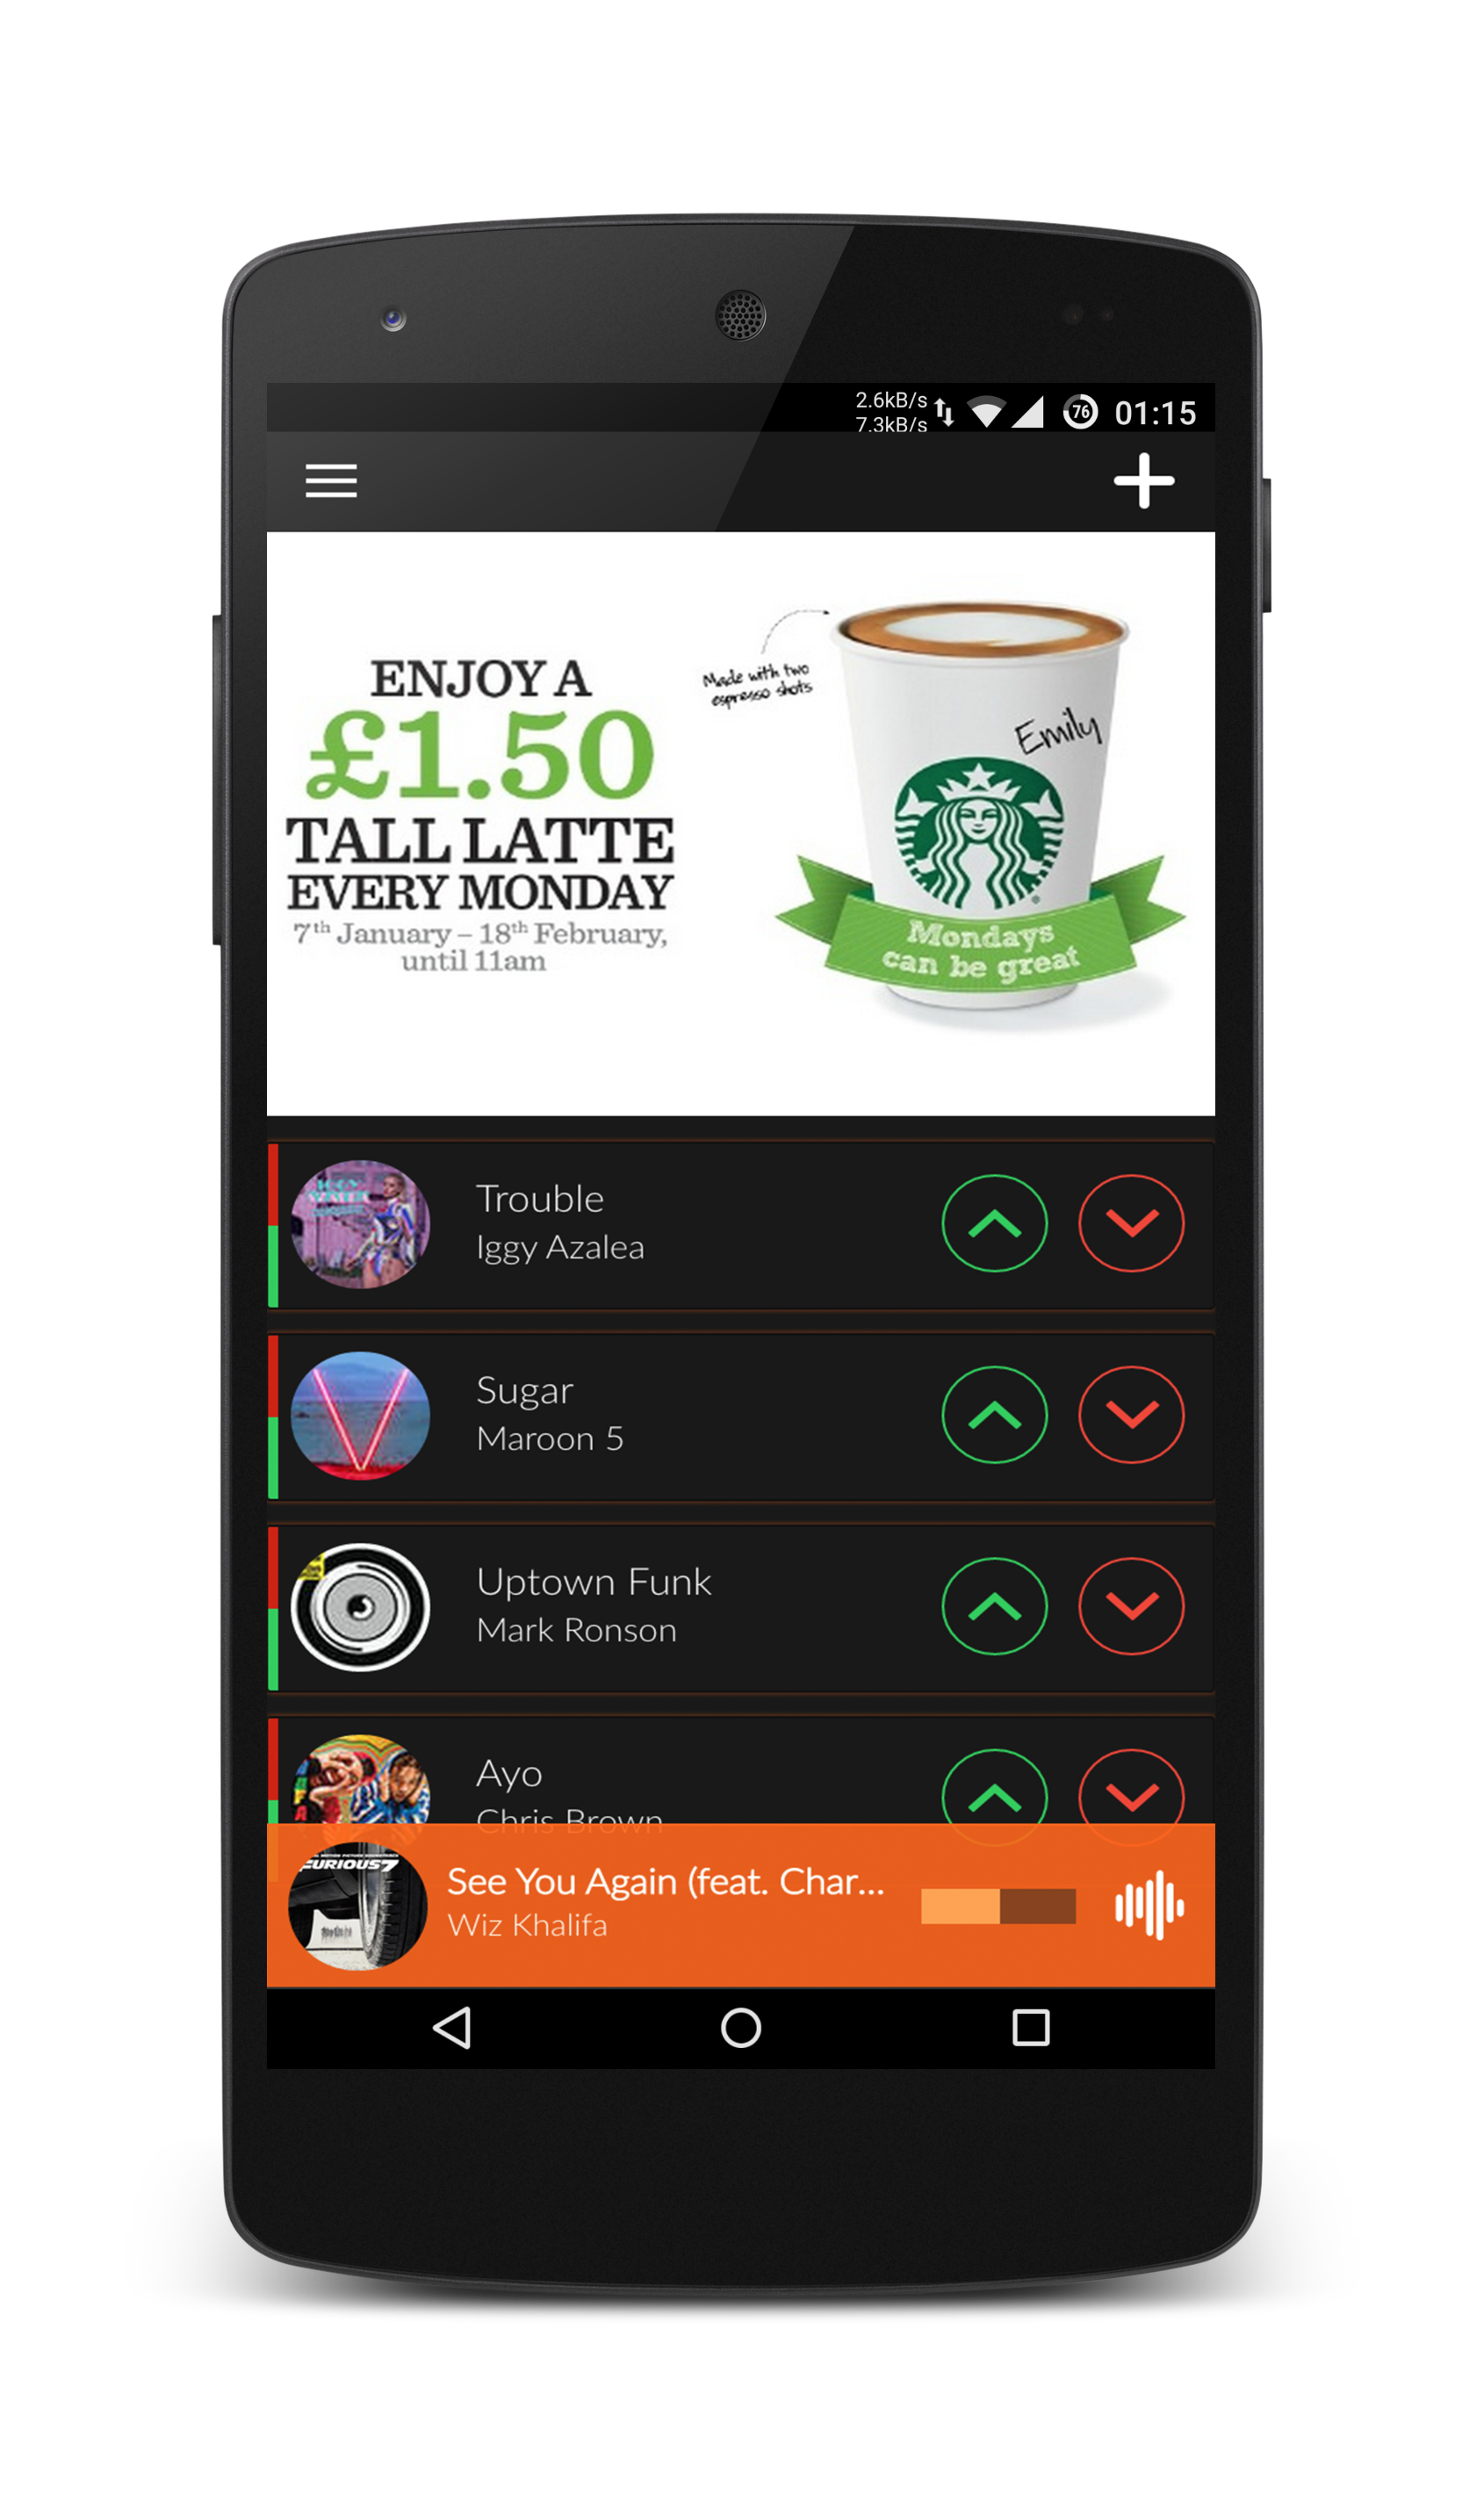
\includegraphics[width=0.3\textwidth]{./img/idea_user_prop.png}
\captionof{figure}{This is the playlist part of the app where users can add their favourite songs as well as up-vote and down-vote any songs within the playlist.}
\label{fig:image_user_prop}
\end{minipage}\\

\subsection{Business Value Proposition}
We have carried out a value proposition for the business and this follows the same structure as the user value proposal.\\

\textbf{(1)} Choona is a music-sharing app that allows customers to collaboratively listen, interact and suggest music in your retail space or business premises through the cloud-driven system.  \\

\textbf{(2)} Choona offers the business a way to enhance a customers experience.  Allowing customers to listen to their favourite music is a sure way of making sure they stay longer and that they make more purchases.  It is also a great way to advertise (via images and sound bites) new products and special offers that may otherwise go unnoticed.  \\

\textbf{(3)} There are several key benefits to Choona for the business:
\begin{itemize}
\item Customers may stay longer thus increasing the number of purchases they make; this increases sales and profit.
\item Advertisments will also gain increased product interest and increased sales revenue
\item Data analytics - Choona will collect endless amounts of data that can then be analysed to find trends or relationships that help the business improve in any area it wants/needs.  
\item The business has an increased/new online presence through the social media activity feature. 
\item Businesses can taylor their default playlist to music that suits their target audience thus making sure they attract the right customers.
\end{itemize} 

\textbf{(4)}\\
\begin{minipage}{\linewidth}
\centering
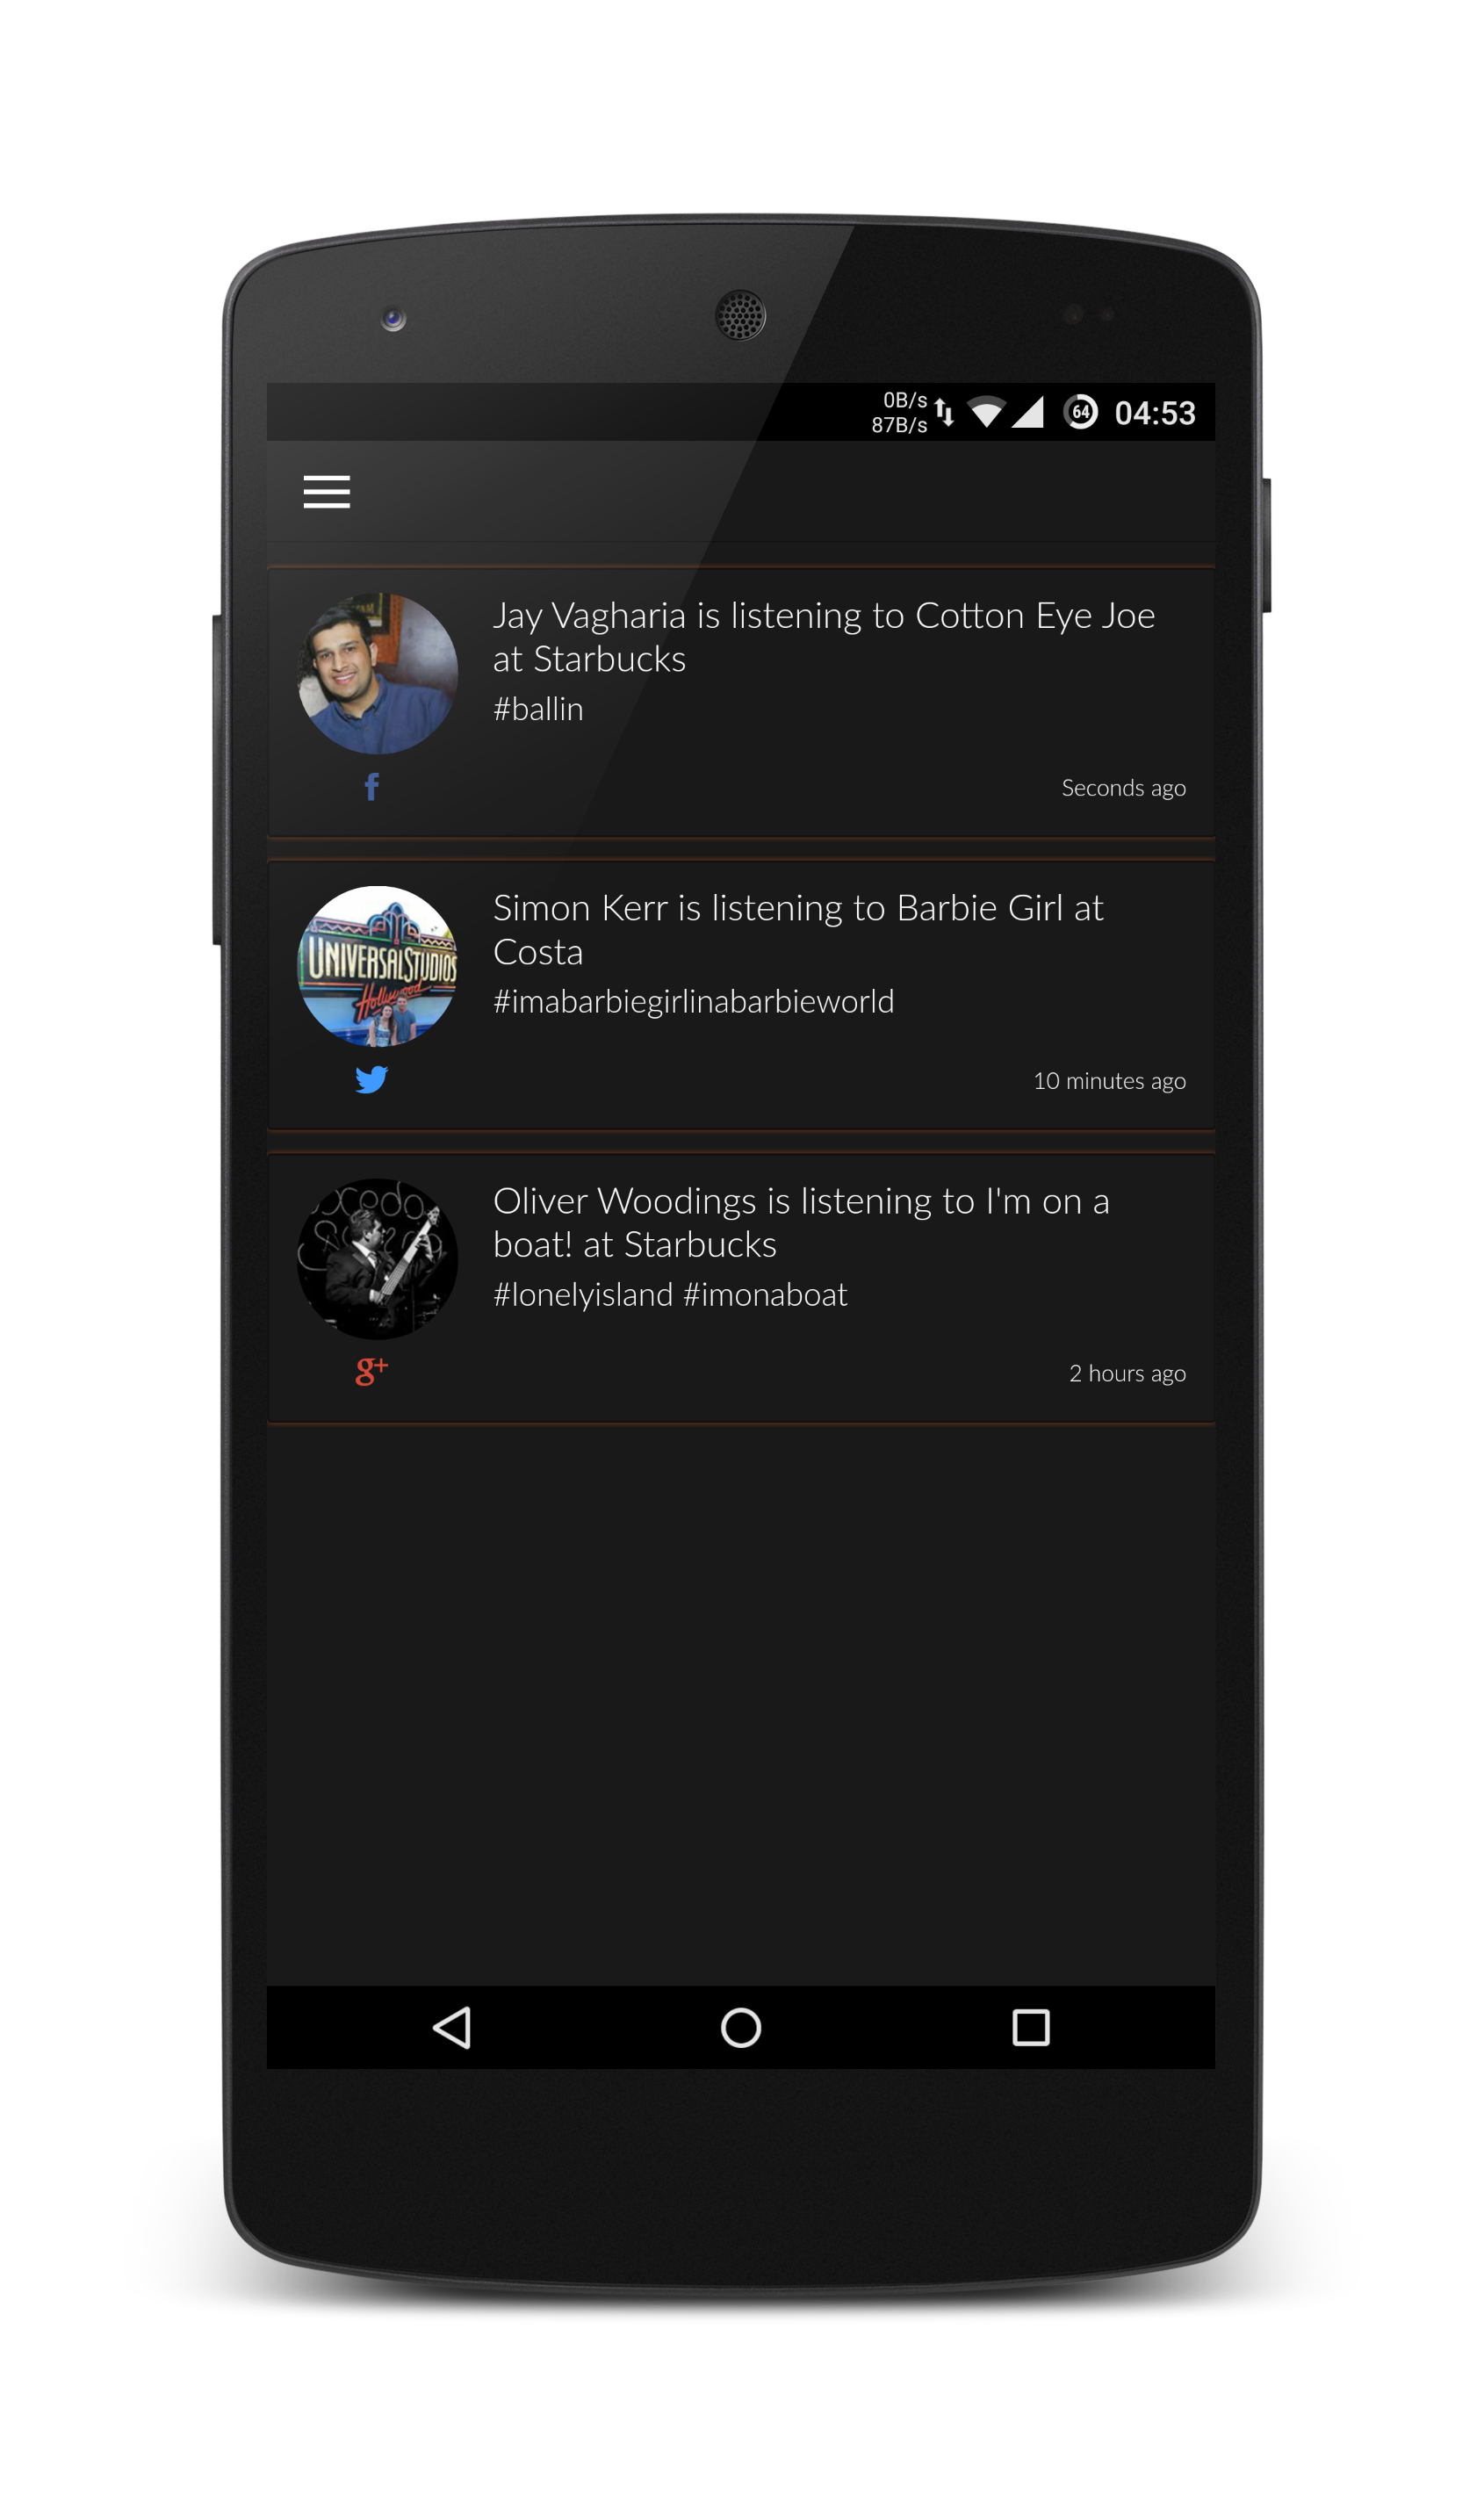
\includegraphics[width=0.3\textwidth]{./img/idea_bus_prop.png}
\captionof{figure}{This is the activity page; this is where the online presence of the business starts to grow.  Please refer to figure ~\ref{fig:image_user_prop} for a look at the placement of image adverts.}
\label{fig:image_bus_prop}
\end{minipage}\\

\subsection{Business Model}
As part of the business plan, we created a lean canvas.  This is shown below; and depicts how we aim to bring success with Choona.\\

\noindent\makebox[\textwidth][c]{%
\begin{minipage}{\linewidth}
\centering
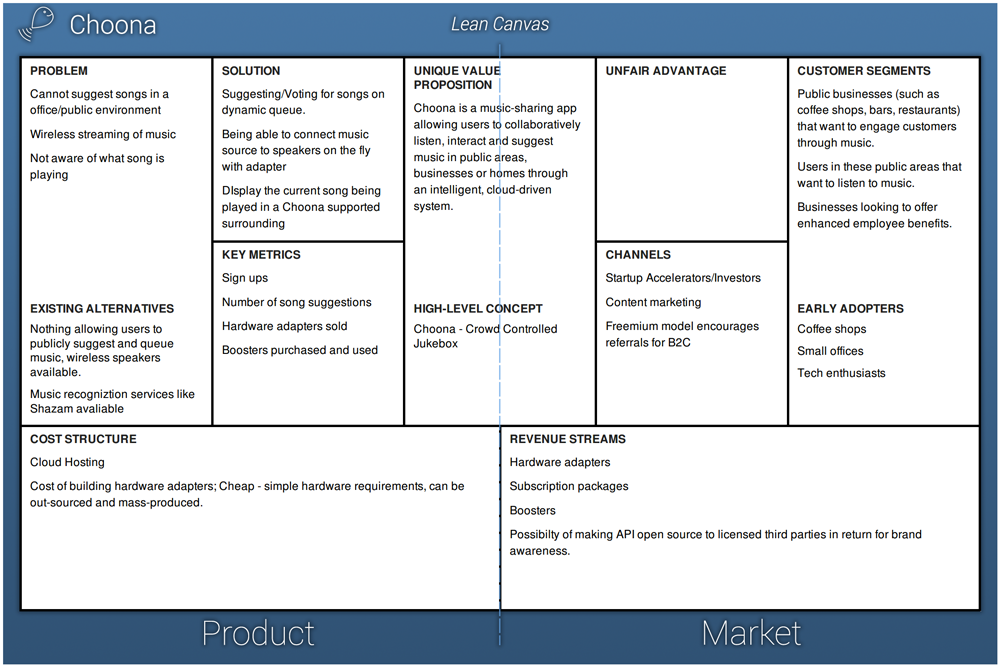
\includegraphics[width=1.0\textwidth]{./img/lean-canvas.png}
\captionof{figure}{This lean canvas has taken inspiration from Peter Drucker and his theories on firms as well as aspects of Michael Porter's value chain maps.}
\label{fig:lean_canvas}
\end{minipage}}\\

\subsubsection{The problem solved?}
At the moment, there is no service that provides users with the ability to select the music they listen to in public areas and the office.  Choona provides them with this ability through a simple mobile facing app that interacts with a system connected to the cloud.   \\

\subsubsection{B2B}
The B2B model essentially means we are providing a product or service to a business.  We are providing businesses with the ability to offer Choona to their customers.  An administration account will be provided that finds their music source(s) and makes it available for customer access.  This account will be allocated a certain number of user connections based upon the subscription package they purchase.  The business will have access to define a default playlist; playing when no other songs have been added by customers.  Businesses will also be able to advertise to customers, whether it be via images on the customer facing app or via sound bites that are inserted between songs.  \\
There will be several different subscription packages available for the business to subscribe to.  The larger the business (whether that be across one location or multiple locations), the more connections they will want to have.  A large organisation will have two levels of management; management across the overall Choona account and management for each different Choona location.  Regardless of this, there will be a standard offering of packages and these are outlined in figure ~\ref{fig:sub_packages}.  \\

\noindent\makebox[\textwidth][c]{%
\begin{minipage}{\linewidth}
\centering
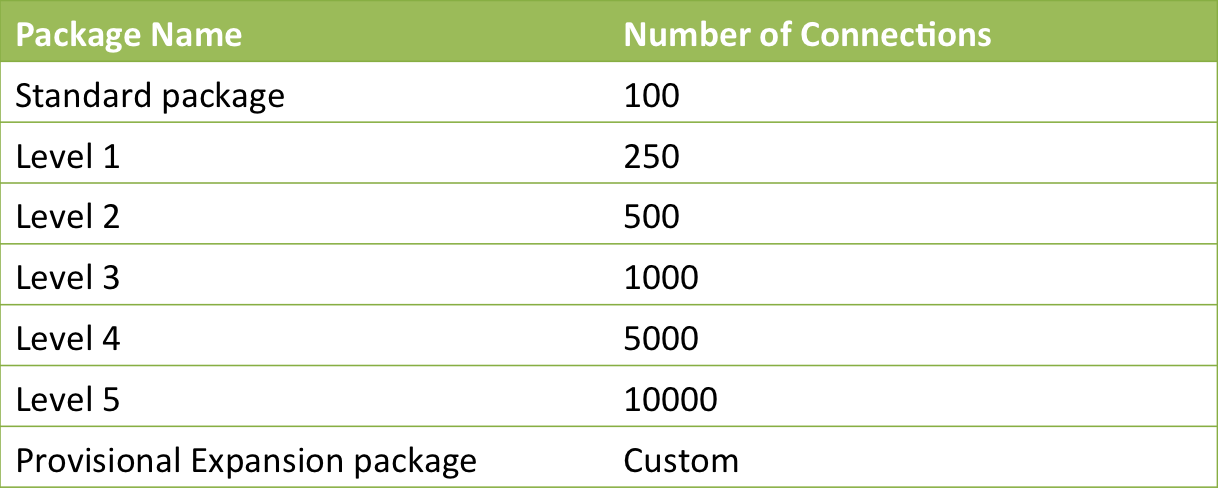
\includegraphics[width=0.8\textwidth]{./img/b2b.png}
\captionof{figure}{Subscription packages}
\label{fig:sub_packages}
\end{minipage}}\\

Unfortunately, we have not had enough time to carry out cost analysis and therefore we cannot put a price beside these packages.  A detailed research analysis of the market will have to be carried out before we can make such estimations.  We do however have a outline on what each package offers; number of connections.  The standard package is a very small package and is aimed at small businesses.  This will be a free package as we plan to adopt a freemium model.  A freemium model is one where core functionality is given away for free but the premium product is sold for a price.  The reason behind using this approach is that it should promote brand awareness and entice more businesses to offer Choona and entice more customers to use it.  \\
In the B2B model, a small number of connections will be given away but in order for the business to allow more customers to use the service, they will have to pay for any additional connections (through upgrading their packages).  The premium packages move from Level 1 to Level 5 and range from 250 connections to 10000 connections. These packages have been created based on several different sources and the information they have provided.  Firstly, according to business insider, Starbucks have around 625 customers per day per store\footcite{starbucks} across 750 stores in the UK\footcite{starbucks_more}.  Therefore, across the UK per hour, they are server over 43000 customers.  This is a huge number and therefore a large connection package would be needed to offer Choona to all customer.  This is why we have created Level 5 package.  Based upon the figures from JS Sainsburys\footcite{sainsburys}, they carry out around 119 transactions per hour per store.  This is a significant number and with more than 1200 stores across the UK, they too need a large number of connections.  We have also spoken to a member of the Loughborough Students Union.  On hearsay, they have estimated the average number of people on a night out to be around 4500.  Over the course of a 6 hour night, this would fluctuate somewhat but at anyone time, the average number of customer would remain around 2000 people.  This has resulted in package levels 3 and 4.  Packages 1 and two have been created for the purposes of smaller businesses that have one, maybe two locations and for large businesses that would use Choona as an internal music application.  Provisional expansion packages are for the one-off occasions where it is not necessary to have the package for a specific length of time.  Concerts are a great example, they happen over a 1, 2 or 3 day period.  Rather than miss out on the Choona experience, we can offer a package that matches the event in terms of duration and number of connections; its a win-win for both the business and for Choona.\\
The second part to the premium side of the freemium model is the sale of a physical adaptor.  This can be purchased as another method of connecting to the cloud and streaming music.  Businesses may want to purchase such hardware whenever laptops and computers are not readily available. \\

\subsubsection{B2C}
B2C covers the private use of Choona within one location and for a non-commercial use.  This covers private parties and normal day to day use between yourself and immediate family within the home.  The B2C model is similar to the B2B model in that it will follow the freemium model.  The user will have free access to the Choona app where they can use it in different Choona locations.  Whenever they want to privatise and create their own Choona location, they have to subscribe for a standard package; this will be free.  However this offers a very small number of connections (5).  If they wish to increase their number of connections, they can upgrade to a higher package.  At this moment in time, we have not been able to do any research towards this type of subscription and therefore we cannot outline package levels or number of connections within these packages.  \\

\subsubsection{Subscription Model}
As we identified in both the B2B and B2C models, we will adopt \emph{subscription commerce}.  On a monthly/yearly basis, the businesses subscription will be renewed and a fee will be paid to Choona.  There are numerous benefits for adopting such a model.  For the business, they will never have to remember to reorder every month; which provides them with the piece of mind that they will receive exactly what they have signed up for.  It is also good for Choona as this will provide us with a constant revenue stream.  We won't need to be constantly bring them through a `checkout' process. 
Secondly, subscription based services are generally a novel idea within their market.  The novelty alone will create a good deal of publicity and drive sales without the need for large volumes of publicity.  \\
It is important to consider the subscription length because a longer average will increase the Customer Lifetime Value.  In doing so, Choona will maintain an increased profitability rate due to the retention of customers and businesses.  This will result in us being able to pay more (through advertising and personalised subscription packages) to sign up further businesses and customers.\\

  \clearpage
  \section{Literature Review}

\subsection{User Interface Design}
Having read different articles relating to Human Computer Interaction components, several factors have been identified that directly link to improving interfaces of mobile applications.  Some of these are the use of graphics, colour, font and other effects.  \\
\textbf{Colour} is one of the main attributes and it covers many different areas including background, text colour and visual effects.  Lets first consider background and text colour.  There is a lot of different opinions on this topic; a lot of people will lean towards a light background with dark text.  Dark backgrounds (dark designs) are becoming very popular now and add a creative and elegant appeal to the app.  This is not something that can be left to preference.  There are situations when dark backgrounds suit the app and there are situations when a light background is preferred.  An app with lots of reading is better off having a light background with dark text.  A recent survey was taken on this area and 47\% prefer light background because it aids with \emph{readability}.   Another 10\% said they prefer dark backgrounds with 36\% saying it just depends on the function of the app\footcite{dark-web-design}.  With our app in mind, we are not so hung up on readability but eye fatigue.  We want the user to be able to use the app in any conditions whether it be during the day, night, in unilluminated rooms (bars and nightclubs) or illuminated rooms.  With this criteria in mind, we need to consider something that has not too high-contrast.  We do not want a full white on full black or vice versa.  We can use dark grey with off white and this will prevent the eyes burning out.  One final note to make; darker backgrounds tend to use less battery.  A test was carried out on an AMOLED screen and the results showed that `mostly' white background use 1/3 more battery than black backgrounds\footcite{dark-power}.  Another test was carried out on a Nokia Lumia 720 (with WVGA IPS screen) and this used 6.37\% more battery having a white background compared to dark background\footcite{battery}.  \\
Now if we have the dark grey background, we need to consider other colours to use with the app.  Blue is usually a popular colour of choice (the world's favourite)\footcite{blue}.  Blue is the colour of the intellect and the mind.  However, blue can be difficult to see on certain backgrounds as it tends to blend in.  This is actually to do with our eyes.  There are fewer photoreceptors that react to blue compared to other colours and they are not in the centre of the retina because it is sometimes hard to distinguish.  \\
Lets consider another colour; orange is included in Ubuntu's colour palette as they believe it signifies a community feeling.  There are many other descriptions of orange - it is classified as a warm colour, it radiates warmth and is often associated with energy, happiness, attraction, stimulation and comfort\footcite{market-share}.  We want our app to have a community like feeling.  This is an app for the public where they can talk through the language of music.  Two other interesting words here are \emph{attraction} and \emph{stimulation}.  Ultimately we want users to be attracted to our app, enjoy their experience and to keep using it.  Although colour won't have too big an emphasis on this, a well designed app can and colour plays a part in this.  Therefore orange seems to be a good colour choice.  
Colour can also used to convey information through visual recognition.  A colour like green means on, safe, valid etc while red means off, danger, invalid etc.  We can make use of these colours in our app to provide information to the user.  \\
Talking of colour, one of the most important thing to remember is to not use too many different colours.  We want to keep the colour scheme minimal.  A busy colour scheme will obscure the dark background as the contrast will be too sharp.  Therefore we shall stick with 2 different colours and a background colour.  \\

\textbf{Font} is another important consideration.  It is important to make sure the selected font is clean, crisp and works well with colours we have chosen.  There are several areas to consider here; the first being weights.  If we want to try and create contract and a visual hierarchy within the app, we can consider different weights such as light, normal, italics, bold and extra bold.  Legibility is also important due to the number of small scree devices there are currently on the market.  If we use a font that is hard to read when it is smaller, then our app design has a serious flaw.  Therefore it is important to use a \emph{sans serif font}.  This type of font does work well with a dark background.  
he trick, though, is to put only larger text in serif fonts, so that the extra white space floods around each character and makes the text very legible.  \\
There are several other key considerations.  Consistency; the app should be as consistent as possible with commands and menus containing the same content and format.  If there are buttons or features designed on one part of the app that act in a certain way, then if this button/feature appears somewhere else, it should act the same way.  The app must be navigable in the sense that we can manoeuvre between the different pages.  Any messages that are displayed (toast notifications etc) should be descriptive and helpful.  Simplicity is also very important and ensures the user will keep coming back to the app.  Many useful apps have been created over the years yet people do not come back because they find it awkward to use or they find it complicated to use.  An example of this is Bump.  When this was first released, it had features to transfer music, photos, contact information other documents and recommended apps.  But due to its complicated nature, it was slated and users abandoned it.  When the creators re-developed the app with simpler page layouts, the app became easy to navigated and simple to understand.  That is when its potential was realised and now has been downloaded millions of times.  

\subsection{App Development}
For the purposes of our prototype, it would be too time consuming to consider native app development therefore we need to consider using frameworks.  Firstly, there is \textbf{PhoneGap}.  PhoneGap works across multiple platforms (iOS, Android, Windows etc.).  Currently, the UK operating system split is 49.7\% android and 42.5\% iOS with the remaining percentage covering Windows, Blackberry and others\footcite{market-share}.  The market is dominated equally by both android and iOS therefore choosing to create a native app on either one of these OS's rules out a large user base thus using Phonegap guarantees we have an app for both types of devices.  \\
If we go one step further, we can look at \textbf{Ionic}.  The creators of \textbf{Ionic} said they have focused on performance.  In doing so, they have brought about simplicity - it keeps a flat, clean simple and powerful UI without unnecessary rendering of rounded corners etc.  This fits in with our idea of the app; we want something simple and clean as this will result in a better user experience which will entice the user to use it again.  

\subsection{Effects of Music}
Music comes in very different forms and covers many different genres.  This leaves it very hard to play music that suits most or all kinds of customers.  According to ``Which'', its not actually the music we like that grabs our attention but its the music we don't like that we notice most.   Therefore, we don't want people to be listening to music they don't like for one main reason; it will annoy them and potentially make them leave the facility.  \\

Music has a lot of power; it moves people of all cultures.  Unfortunately, it is not understood as to why listening to music triggers such a rewarding experience but through brain scans, it seems songs trigger the same brain flooding (with dopamine) as food and sex.  This reaction then causes the Nucleus Accumbens to communicate with the temporal gyrus\footcite{love-music}.  This causes us to register memories; we have a likeness to remember the fond memories with links of music and sounds.  Having this knowledge, we can use this to stimulate customers; happy customers drawing on happy memories will result in many different activities and these should be mainly positive ones for the shop, whether it be more purchases or decisive purchases.  \\

How music is played also has an effect on our activities within a shop.  There have been several different studies carried out over the years linked to how volume, speed and type of music effects our behaviour.  For instance, the louder the music, the more likely it is that people will spend less time in that shop\footcite{annoying-music}.  There are cases when this is a good thing; both for the customer and for the business.  Lets consider a supermarket.  Before we make our way to the supermarket, we have a fairly good idea of what we want.  Therefore we are not actually going to spend any less money if we are fast and efficient compared with spending more time in the store.  Its good for the customer because we will have more time to spend on other activities and its good for the business because their stores do not become bunged and they should have a steadier stream of customers.  \\
Slower music will result in customers spending more time in store and hopefully an increase in purchases\footcite{annoying-music}.  This type of scenario is what businesses want when customers come for a look around e.g. cloths, furniture, jewellery and coffee shops etc.  The customer may not have had the intention of making any purchases but the slow music changed their brain activity that resulted in a purchase they didn't intend to make.  Even in coffee shops, it may result in the customer(s) grabbing another coffee before leaving. \\
Listening to the wrong type of music can make people believe they have been somewhere longer than they have.  Something like this will force the customer to leave the store, maybe even before they have purchased anything.  Therefore having the right type of music playing is essential to keep the customers in the store long enough to make sure they makes purchase.  There is no better way of doing this than allowing the customer to have a say in the music they listen to. 

\subsection{Competitors}
We have taken a look at other apps and services on the market and feel that nothing matches our idea. The closest service available is from \textbf{Sonos}. Sonos is a smart system of speakers and audio components that unite your digital music collection in one app and can then be controlled from any device. The rise of digital music has allowed for us to bring our music wherever we go, through media such as iPods, MP3 players etc. However, there hasn't been the same advancements in terms of systems that don't move around. `Wireless' is the word that comes to mind when thinking of a solution. It is now possible to stream audio to a wireless device (speaker) and without compromising on the sound quality. Sonos provides the user with the ability to play music from a device wirelessly anywhere in the \textbf{home}. However, there are two issues with this; it is only available for the \textbf{home} and the consumer needs to purchase expensive \textbf{hardware}. The cheapest speaker available for purchase is \pounds169. If you are a music-orientated person, you may wish to purchase their high-end hardware which can cost up to \pounds1200. Unfortunately, Sonos do not support other wireless speakers. An adaptor can be purchased to allow these to be connected to their system, the \emph{Connect} device, but this costs \pounds279.  

\textbf{Pure} have also moved into this market where they provide wireless speakers and hardware for \emph{wireless music} in the \textbf{home}. They also allow you to purchase hardware to link your current speakers with their system at \pounds69.  This is much cheaper than Sonos but is still quite expensive. It allows the consumer to wirelessly play their music from any music app or streaming service they want. \textbf{Bose} also provide a very similar service to Pure, but the hardware costs are more expensive.

From this, we can see that there are no services available for the wireless sharing of music outside the home. Our app would unite music into anybody's daily routine, whether this is at the office, coffee shop, restaurant as well as the home. We also want to make sure that no expensive costs are applied.
Competitors can appear at anytime during the development of a project, so it is important that we keep looking for emerging competitors and that we can identify how our product is unique to theirs. 

\subsection{Music Sources}
In today's market, there are many music sources available to an individual. We have virtual music from services such as `Spotify', `Google Music' and `iTunes' as well as physical music on `iPods', `MP3 players' and other hardware devices. \\

\textbf{Spotify} is a music streaming service that offers access to a library of over 20 million music tracks with over 40 million active users. It is available across 58 markets including the UK, USA, France, Germany, Hong Kong and Argentina. It is available on iOS, Android, Windows phone as well as PC and Mac. One chain that is affiliated with Spotify is Costa. Costa have their own playlist that people can access from their device. \\
\textbf{Google Music} is another streaming service and offers the same service as Spotify. Again, they have a large library of songs (around 18 million) and the service is available in over 57 countries on all Android devices as well as web browsers. \\
\textbf{Auracle Music} is a custom streaming service that delivers the best background music through the internet.  This allows you to tailor the music you have playing to suit your needs.  At the moment, this system contains over 30 different licensed music channels with a whole host of music making it compatible with this project.  The top advantage of this is actually the fact that it is for commercial use.  This therefore means we can use it alongside Choona and not require any further licenses.  \\
A year ago, Apple's \textbf{iTunes} accounted for 75\% of the digital music market and with a huge 575 million active users. Although this may have decreased slightly in the last year, that is still a large user base. As well as general users, Starbucks is affiliated with iTunes and use this service to hand-pick and play music throughout their stores. The idea of allowing customers to put forward their music preference may be of interest to a chain like Starbucks amongst others. 
The issue with iTunes is that all the music has to be purchased before it can be listened to.  There is no monthly subscription fee where you can listen to as much or as little music as possible.  Apple are however brining out their own music streaming service; called \textbf{Beats Music}.    
The above figures suggest that the music streaming industry is vast and that music is a part of many people's lives. Coffee shops have integrated these sources and music into their environment, but without the customer interaction. Choona would provide this interaction. Over the course of this project, we shall identify more sources because having more sources creates a larger user base as well as a better music library. We shall look at how the different sources work to try and make sure we have adaptors in place that can cover the wide variety of sources available. 

\subsection{Legal Issues}
With this type of app, there are certain laws and legislation in place that have to be adhered to in order to play music in public.  
\subsubsection{Public Performance License}
    Music playing for customers or staff through media such as radio, MP3, TV etc. is considered a \emph{public performance}. The \emph{Copyright, Designs and Patents Act 1988} means that an agreement is needed from the copyright owner before the material can be played in public. A music license (PPL) will grant this agreement. In most cases, a license is required but there are a few instances when one is not required. One example of this is where PRS  artists have waived their rights. PRS for Music represents the rights of over 100,000 artists in the UK.  It provides licensing to organisations to allow the playing, performing and availability of copyright music on behalf of the artists and overseas societies.  The royalties are distributed fairly and efficiently.  Another example is a hotel, guest house or B\&B that has fewer than 25 rooms with no areas open to non-residents. 
    Any business such as a coffee shop, bar or gym that plays recorded music in public will legally require a PPL. The likelihood of our service being used in places that don't have a PPL and require one is small.  Most coffee shops, restaurants, gyms etc. will already have the license in place.  It will be work places deciding to implement our service that will have to go about retrieving a PPL.\\
The costs vary depending on the facility and how the music is used.  Cafe's, restaurants, pubs and bars are charged based on the area size, so the smaller the area, the smaller the fee.  This is an annual fee and ranges from between around £130 to £325 per year\footcite{ppl}.  The reason the fee is not too large is because the music is just background noise and therefore it is not the main attraction.  In some establishments, they may not play background music and so if they wanted Choona, they will have to apply for the license.  Ultimately, it will be there decision as to whether they decide to take on this extra annual fee; maybe Choona can promote them enough to gain extra sales thus warranting its purchase.    \\
\textbf{Retail shops} too have to pay a fee and again this is based upon the area size of the store.  These range anywhere from around £130 to £220.  A lot of retailer space does not have music in the background and so they will need to judge whether or not they want to take on Choona and the required licenses they would need. It is all about whether or not Choona as a service will provide enough benefits over the costs needed.  If the store already has a license in agreement, then the integration of Choona should be simple.  \\
\textbf{Nightclubs} have a different payment scheme; they have a standard fee to pay and on top of that, they pay an additional cost (for each night of entertainment) that is calculated depending on the number of customers (population size) and the number of hours the music will be played\footcite{ppl}.  Therefore fees can escalate enormously over a year long period.  This though however would not make any difference for them; they will have to pay these fees regardless of whether Choona is integrated or not therefore integration should be simple and straightforward.  
There are tables highlighting these costs for the different premises and these are available in the Appendix.  
      
\subsubsection{Entertainment Licensing}   
Introduced on 6 April 2015, this licence may need to be acquired by businesses, organisations and even individuals who want to provide entertainment.  This entertainment can cover more than music but for this project, we only want to consider the instances when the entertainment revolves around the playing of music or the performance of music.  This license will apply to places such as night clubs, live music venues (concerts) and large indoor arena's.\\
Below are the set of conditions where if any are met, a license is required:
\begin{itemize}
\item Entertainment is provided between 11pm and 8am
\item Amplified live/recorded music performed to an audience greater than 500 people
\item Recorded music played to an audience on premises where the sale of alcohol is not licensed.
\end{itemize}
This covers bars, nightclubs, concerts and other different use cases for Choona.  The fees have been laid out in figure \ref{fig:license_prices}.\\ 

\begin{minipage}{\linewidth}
\centering
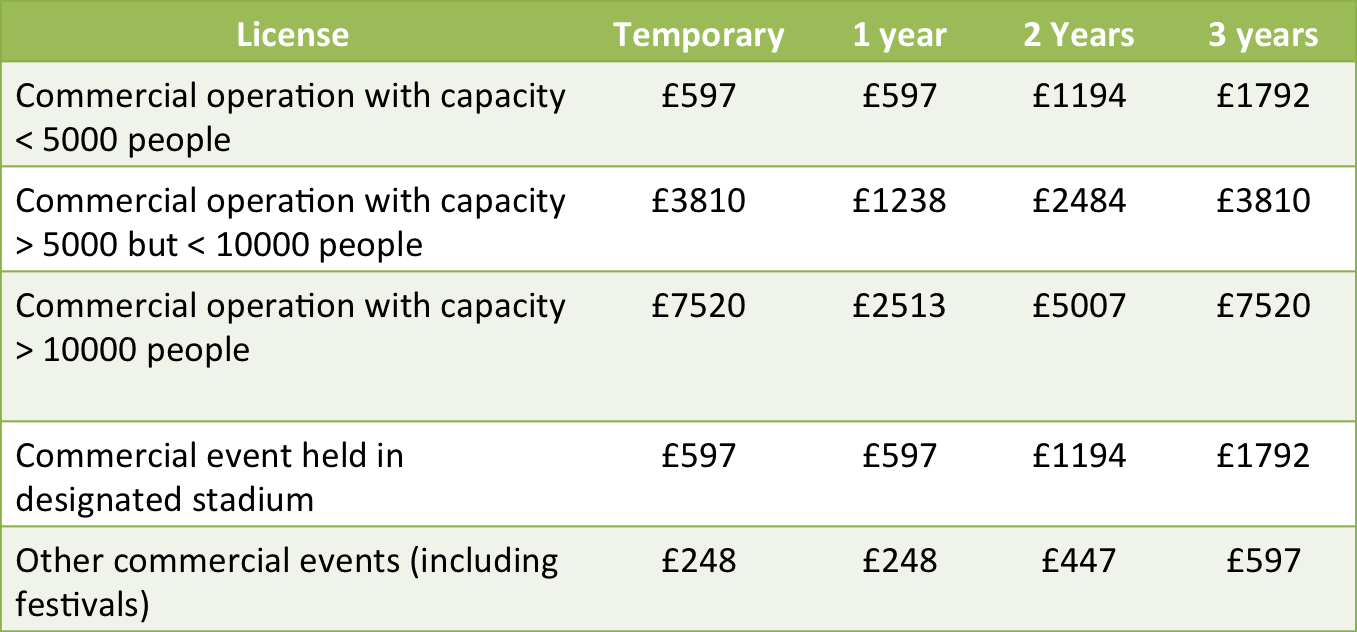
\includegraphics[width=0.8\textwidth]{./img/table_license.png}
\captionof{figure}{Example entertainment license pricing scheme\footcite{license-section}}
\label{fig:license_prices}
\end{minipage}\\

The prices vary somewhat and for the larger events and locations, these prices may not be too much of a concern.  However, when it comes to smaller venues, they may be reluctant to pay the fee.  The process itself in order to get a license, an application is to be submitted.  The application can be considered for a period of 6 months before a decision needs to be made.   This is not a short process and therefore if Choona is to be implemented in certain establishments, the appropriate amount of notice needs to be given so the license can be granted.  

\subsubsection{Music}
At this current moment in time, Spotify is for personal use only.  Therefore we cannot make use of Spotify as a commercial source due to their terms of service stating that ``Anywhere you need a license to play music, you are not allowed to use Spotify''.  Obviously this is a big issue and something that has to be considered deeply.  There are some small services out there that do allow for commercial use of music streaming (something like Auricle Music) but these are not on the same level as Spotify, Google Music etc.  \\
\textbf{Beats Music} is also for personal/private use only.  There is slight leeway here because unlike Spotify, there allow for commercial use if the user is a curator.  In there case, a curator is someone who has a customised profile page that contains authentic postings and curated playlists.  This will have to be verified with Beats Music.  This could actually allow Choona to create this type of profile and eventually make use of this streaming service as the source.  

\subsection{Geolocation}
\textbf{Geolocation} is a technology solution used to identify the real-world geographic location of an object.  Geolocation makes it possible, from a device connected to the Internet, to obtain various types of information in real time and locate it on the map with high accuracy at a given point in time. 
Many different methods can be used to collect this data but for the purposes of this app, it will be through mobile phones (users device containing the app) and IP addresses (for the Choona service end).  \\
The idea behind geolocation within this project would be to connect the user to the Choona system within their location automatically or show the different Choona locations within their geofence so they can choose which one they want to connect to.  In doing so, we are highlighting Choona locations that are within range only thus limiting the search area and making life simpler for the user.  There are several advantages to Geolocation.  First of all, we can have \textbf{targeted adverts}.  For both the customer and the business running Choona, more locally-targeted adverts can create a better app experience.  Customers will get adverts related to their location and not just any old adverts thus the experience will feel less spammy.  For the businesses, they can use this space to advertise new products, special offers in order to improve sales and custom.  \\
Secondly, Geolocation can help improve user profiles.  We can understand exactly where a user is in terms of activity and thus we use this to promote new app features or create different features based on user preferences.  Things to consider here would be algorithms that automatically indicate songs you can play based on previous songs you have added to playlists.  We can also use this to send push notifications; the sending of messages that could be linked with Choona in general or a specific Choona location.  It is reasonably simple to implement the basic functionality of Geolocation on the app side with use HTML and JavaScript needed but to get it working with the backend will require considerable work and time to make it effective and consistent. 

\subsection{NFC}
Near-Field Communication (NFC) is a form of short range wireless communication (4cm or less to launch a connection) allowing for radio communication and the passing of data packets between two devices, or smart tags that work with NFC. NFC is an advancement to RFID systems because it allows for two-way communication. This two-way communication can then be used for authentication purposes or data exchange. \\
At the moment, not all devices support NFC and it is suggested around 20\% of phones worldwide will have NFC capability by the end of 2014. This figure is set to increase dramatically over the next five years meaning more devices will have the capability and more users will be familiar with the technology. This widespread reach of NFC phones could mean one day that NFC tags become as common as bar codes, so it makes sense to make use of this technology.\\

Using NFC tags with a mobile device, a user could access the playlist at their current location without the need to search for it. The idea is very durable as NFC tags are small and cheap enough to integrate anywhere. They do not need a power source but instead draw power from the device that reads them. \\

\subsubsection{Viability}
With NFC, it is unfortunate that apple devices cannot use it.  Some do have NFC functionality but this is just for the purpose of `Apple Pay' and nothing else.  Almost all android devices currently have NFC functionality that can be used by the apps themselves.  NFC tags or stickers are extremely cheap; around £1 per tag.  In bulk purchases, this will decrease dramatically.  They are extremely easy to encode through a NFC enabled device and allows for protection to stop it being changed by unauthorised user.  If we were to adapt the use of NFC, the business themselves should be able to encode the tags themselves.  It may be an idea to have a tutorial available where the business just needs to follow the small number of steps involved.\\
    
  \clearpage
  \section{Requirements}

\subsection*{Global}

\noindent
\begin{tabular}{|l || p{12.0cm}|}
  \hline
  Requirement:       & REQ.1 \\ \hline
  Type:              & Functional \\ \hline
  Description:       & The user must be able to connect to the geolocation configured by the client. \\ \hline
  Rationale:         & When the system is initially set up, the client (coffee shop, office etc) will set up a geolocation and geofence for their customers using choona. The user will then be able to connect to this geo-area via their phone and then be able to suggest songs for the public in that geofence. This must be paired with REQ.2 for the user to get full access to the app. \\ \hline
  Dependencies:      & REQ.2 \\ \hline
  MoSCoW Rating:     & Must \\
\hline
\end{tabular}\\

\vspace{0.5cm}

\noindent
\begin{tabular}{|l || p{12.0cm}|}
  \hline
  Requirement:       & REQ.2 \\ \hline
  Type:              & Functional \\ \hline
  Description:       & The user must be able to log on using social networks/by email. \\ \hline
  Rationale:         & An account is required for the user to suggest songs. This must be paired with REQ.1 for the user to get full access to the app. \\ \hline
  Dependencies:      & REQ.1 \\ \hline
  MoSCoW Rating:     & Must \\
\hline
\end{tabular}\\

\vspace{0.5cm}

\noindent
\begin{tabular}{|l || p{12.0cm}|}
  \hline
  Requirement:       & REQ.3 \\ \hline
  Type:              & Functional \\ \hline
  Description:       & The client must be able to configure their choona configuration for their customers through a management system. \\ \hline
  Rationale:         & The client must be able to configure different music options for their business and their geofence. This would include things like:
  \begin{itemize}
  \item Subscription options.
  \item Genre restrictions.
  \item Be able to configure any ad services for the location, including sound bytes and carousel images.
  \item Default playlists if no songs are suggested.
  \item Geofence/Geolocation options.
  \item Override the queue if needed.
  \end{itemize}
 \\ \hline
  Dependencies:      & REQ.1 \\ \hline
  MoSCoW Rating:     & Must \\
\hline
\end{tabular}\\

\vspace{0.5cm}
\subsection*{Playlist Page}

\noindent
\begin{tabular}{|l || p{12.0cm}|}
  \hline
  Requirement:       & REQ.4 \\ \hline
  Type:              & Functional \\ \hline
  Description:       & The user must be able to suggest a song using search. \\ \hline
  Rationale:         & For the dynamic playlist to work, the user must be able suggest a song they want to be played in public. This song will then be added to the dynamic playlist ordered by the number of votes. If the song already exists in the playlist then it will not be added again. \\ \hline
  Dependencies:      & REQ.1, REQ.2 \\ \hline
  MoSCoW Rating:     & Must \\
\hline
\end{tabular}\\

\vspace{0.5cm}

\noindent
\begin{tabular}{|l || p{12.0cm}|}
  \hline
  Requirement:       & REQ.5 \\ \hline
  Type:              & Functional \\ \hline
  Description:       & The user must be able to see all the songs suggested by others, managed by an intelligent algorithm for the geolocation they are connected to.\\ \hline
  Rationale:         & The user should be able to see what songs are suggests so they can upvote and downvote; these songs must be sorted by an intelligent algorithm where the amount of votes will be largest variable in maintaining a fair song order (eliminating repetitive or ghost voting). \\ \hline
  Dependencies:      & REQ.1, REQ.2 \\ \hline
  MoSCoW Rating:     & Must \\
\hline
\end{tabular}\\

\vspace{0.5cm}

\noindent
\begin{tabular}{|l || p{12.0cm}|}
  \hline
  Requirement:       & REQ.6 \\ \hline
  Type:              & Functional \\ \hline
  Description:       & The user must be able to vote on the songs suggested by others for the geolocation they are connected to. \\ \hline
  Rationale:         & Songs that are already on the playlist can be upvoted/downvoted by the user. The dynamic playlist is dependent upon this where songs are ordered by a amount of votes. \\ \hline
  Dependencies:      & REQ.1, REQ.2 \\ \hline
  MoSCoW Rating:     & Must \\
\hline
\end{tabular}\\

\vspace{0.5cm}

\noindent
\begin{tabular}{|l || p{12.0cm}|}
  \hline
  Requirement:       & REQ.7 \\ \hline
  Type:              & Functional \\ \hline
  Description:       & For each song, the user must be able to see the album cover, song title and album title. \\ \hline
  Rationale:         & This is needed for the user to identify the song, the album cover adds a visual factor to all the songs. \\ \hline
  Dependencies:      & REQ.1, REQ.2 \\ \hline
  MoSCoW Rating:     & Must \\
\hline
\end{tabular}\\

\vspace{0.5cm}

\noindent
\begin{tabular}{|l || p{12.0cm}|}
  \hline
  Requirement:       & REQ.8 \\ \hline
  Type:              & Functional \\ \hline
  Description:       & The user must be able to see what song is currently playing in the geolocation they are connected to. \\ \hline
  Rationale:         & This is to inform the user what is being played currently. Information such as album art, song title, album title and time elapsed will be shown. \\ \hline
  Dependencies:      & REQ.1, REQ.2 \\ \hline
  MoSCoW Rating:     & Must \\
\hline
\end{tabular}\\

\vspace{0.5cm}

\noindent
\begin{tabular}{|l || p{12.0cm}|}
  \hline
  Requirement:       & REQ.9 \\ \hline
  Type:              & Functional \\ \hline
  Description:       & The user should be able to share the song currently playing.  \\ \hline
  Rationale:         & To add a social side to the application, the user should be able to share what song they are listening to and where on various social networks. Their friends will be able to see this shared information not only on the social networks itself but also on their activity page. They should also be able to add a message to their activity. \\ \hline
  Dependencies:      & REQ.1, REQ.2, REQ.8 \\ \hline
  MoSCoW Rating:     & Should \\ \hline
\end{tabular}\\

\vspace{0.5cm}

\noindent
\begin{tabular}{|l || p{12.0cm}|}
  \hline
  Requirement:       & REQ.10 \\ \hline
  Type:              & Functional \\ \hline
  Description:       & The user should be able to hear the currently playing song through their headphones  in the geolocation they are connected to.  \\ \hline
  Rationale:         & This is for the convenience to the user, they should be able to listen to the music privately if they wish. In some use cases this would be ideal such as in an office environment. \\ \hline
  Dependencies:      & REQ.1, REQ.2 \\ \hline
  MoSCoW Rating:     & Should \\ \hline
\end{tabular}\\

\vspace{0.5cm}

\noindent
\begin{tabular}{|l || p{12.0cm}|}
  \hline
  Requirement:       & REQ.11 \\ \hline
  Type:              & Functional \\ \hline
  Description:       & The user should have the option to buy the currently playing song. \\ \hline
  Rationale:         & If the user likes the song, they should have the option to buy it through various services such as google play, itunes etc. This would also be another technique to monetize the app by promoting the artist and their song.    \\ \hline
  Dependencies:      & REQ.1, REQ.2, REQ.8  \\ \hline
  MoSCoW Rating:     & Should \\ \hline
\end{tabular}\\

\vspace{0.5cm}
\subsection*{Activity Page}

\noindent
\begin{tabular}{|l || p{12.0cm}|}
  \hline
  Requirement:       & REQ.12 \\ \hline
  Type:              & Functional \\ \hline
  Description:       & The user should be able to see a list of “shared” songs.   \\ \hline
  Rationale:         & To add a social side to the application, the user should be able to share what song they are listening to and where on various social networks. Their friends will be able to see this shared information not only on the social networks itself but also on their activity page. \\ \hline
  Dependencies:      & REQ.1, REQ.2, REQ.9 \\ \hline
  MoSCoW Rating:     & Must \\ \hline
\end{tabular}\\

\vspace{0.5cm}

\noindent
\begin{tabular}{|l || p{12.0cm}|}
  \hline
  Requirement:       & REQ.13 \\ \hline
  Type:              & Functional \\ \hline
  Description:       & For each activity the user should be able to see the name of person, the song name and the location the person is listening at together with any additional message and a time stamp.   \\ \hline
  Rationale:         & This information is required for the user to identify each activity and so they can differentiate between their friends. \\ \hline
  Dependencies:      & REQ.1, REQ.2, REQ.9 \\ \hline
  MoSCoW Rating:     & Must \\ \hline
\end{tabular}\\

\vspace{0.5cm}
\subsection*{History Page}

\noindent
\begin{tabular}{|l || p{12.0cm}|}
  \hline
  Requirement:       & REQ.14 \\ \hline
  Type:              & Functional \\ \hline
  Description:       & The user should be able to see the places they visited and the songs that were playing in the time frame they were there.  \\ \hline
  Rationale:         & In the likelihood of the user wondering what song was playing at a certain place they visited and not being able to remember the name, they can use the history page to look up that song.  \\ \hline
  Dependencies:      & REQ.1, REQ.2, REQ.16 \\ \hline
  MoSCoW Rating:     & Must \\ \hline
\end{tabular}\\

\vspace{0.5cm}

\noindent
\begin{tabular}{|l || p{12.0cm}|}
  \hline
  Requirement:       & REQ.15 \\ \hline
  Type:              & Non-Functional \\ \hline
  Description:       & The user should only be able to see history for the last week.   \\ \hline
  Rationale:         & To minimize the data overload on storing all history information for all users. The app will only display history in the last week. \\ \hline
  Dependencies:      & REQ.1, REQ.2, REQ.16 \\ \hline
  MoSCoW Rating:     & Must \\ \hline
\end{tabular}\\

\vspace{0.5cm}
\subsection*{Settings Page}

\noindent
\begin{tabular}{|l || p{12.0cm}|}
  \hline
  Requirement:       & REQ.16 \\ \hline
  Type:              & Functional \\ \hline
  Description:       & The must be able to toggle whether their history will be logged or not.   \\ \hline
  Rationale:         & If the user wishes not to log all the songs played at the places they visited, they should be able to turn this feature off. This would be in the settings page. \\ \hline
  Dependencies:      & REQ.1, REQ.2 \\ \hline
  MoSCoW Rating:     & Must \\ \hline
\end{tabular}\\

\vspace{0.5cm}

\noindent
\begin{tabular}{|l || p{12.0cm}|}
  \hline
  Requirement:       & REQ.17 \\ \hline
  Type:              & Functional \\ \hline
  Description:       & The user must be able to log out from their Choona account.   \\ \hline
  Rationale:         & There should be a button for the user to log out of their Choona account.  \\ \hline
  Dependencies:      & REQ.1, REQ.2 \\ \hline
  MoSCoW Rating:     & Must \\ \hline
\end{tabular}\\

  \clearpage
  \section{Design}

\subsection{System Architecture}

As discussed during the planning stages, Choona will be built using the microservices architecture. Figure \ref{fig:architecture} shows the proposed system design for Choona, split into four layers.

\begin{figure}[h!]
  \centering
  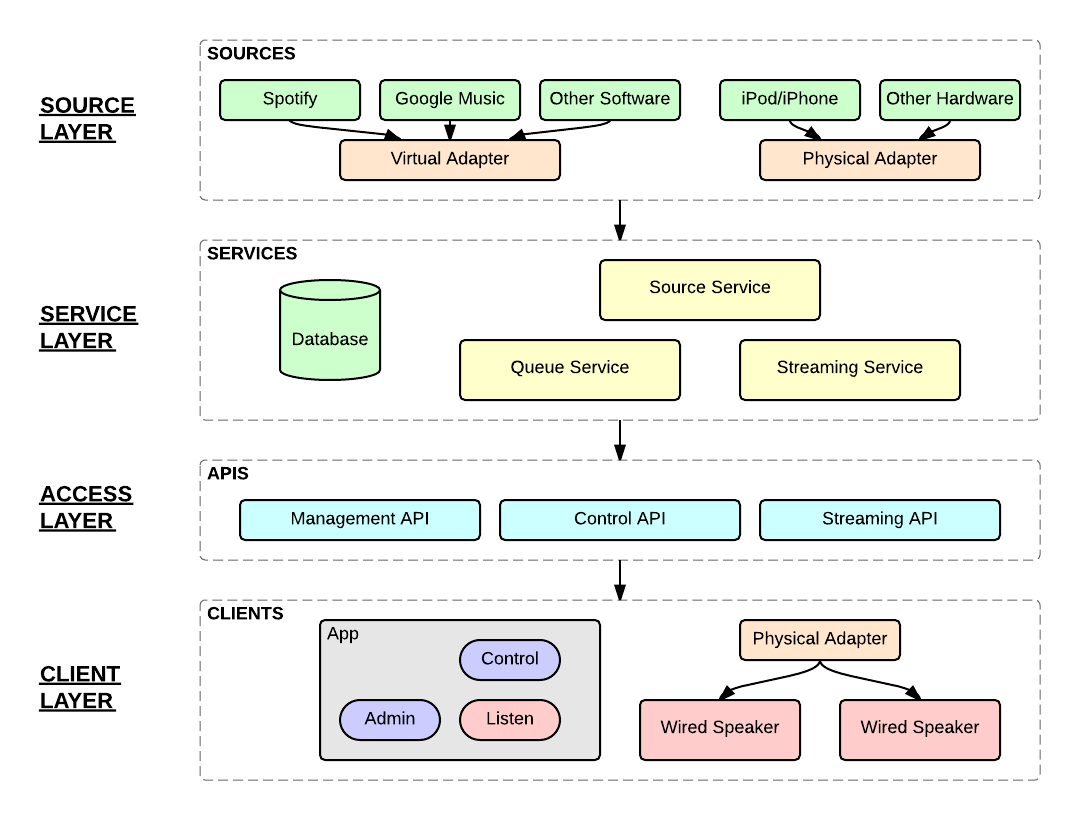
\includegraphics[width=1\textwidth]{./img/sys-architecture.png}
  \caption{Proposed Choona system architecture}
  \label{fig:architecture}
\end{figure}

\begin{itemize}
  \item \textbf{Source Layer}\\
    Sources, such as Spotify and Google Music, all have their own unique APIs. For them to be consumed by Choona they need to present a common interface otherwise other services will need to know how to interact directly with each individual API. Therefore each source will be exposed through either a virtual or physical adapter. Each adapter understands the same set of commands and outputs data in the same format. This means that other services in Choona only need to implement the standard adapter interface in order to communicate with any type of audio source. For the first version of Choona the sources will only need to understand a basic set of instructions:
    \begin{itemize}
      \item \texttt{search [searchString]} - search the source's track database using the supplied search string
      \item \texttt{get [trackId]} - retrieve track information from the source's database for the specified track ID
      \item \texttt{play [trackId]} - stream the audio for the specified track ID
    \end{itemize}

  \item \textbf{Service Layer}\\
    The service layer contains the majority of the \textit{business logic} of the Choona server-side infrastructure. There will be three main services at this layer. The queue service is responsible for maintaining the running playlist of tracks for a particular Choona location. The source service acts as an interface to all the different types of audio sources (instructions documented above). The streaming service takes tracks from the queue service, retrieves the audio via source service and sequences it into a single stream that the APIs can then send to clients. This layer has a more extensive set of instructions:
    \begin{itemize}
      \item \texttt{queue join [locationId] [clientId]} - make a client join a particular location
      \item \texttt{queue add [locationId] [trackId]} - add a song to the queue of a particular location
      \item \texttt{queue upvote [locationId] [trackId]} - upvote a song at a particular location
      \item \texttt{queue downvote [locationId] [trackId]} - downvote a song at a particular location
      \item \texttt{stream add [locationId] [trackId]} - instruct the streaming service to play a particular track next at a certain location
      \item \texttt{stream play [locationId]} - broadcast the stream to all listening clients of a location
    \end{itemize}

  \item \textbf{Access Layer}\\
    The access layer contains APIs that clients can use to interact with the Choona infrastructure. These APIs act as proxies, taking requests from clients and passing them through to the right services in the service layer. The only special instruction the access layer makes available is user authentication verification.

  \item \textbf{Client Layer}\\
    The client layer contains all the consumers of Choona, such as the mobile app and speaker adapter. Clients use the access layer to authenticate and interact with the rest of the Choona infrastructure; they do not need to know about all the individual services, instead they only need to understand the access APIs.
\end{itemize}

\subsection{UI Design}

\subsubsection*{Global Styling}

\noindent\underline{Colour schemes}\newline
There are a number of different colour schemes that can be used for the app, these must be discussed to make sure the most appropriate colour scheme is chosen.  This should line up with our literature and satisfy our target market needs.

To quickly review, as discussed in the literature review a dark user interface is more appropriate for choona because it:
\begin{itemize}
\item Is quite popular, adds a certain elegance to the app.
\item Is more convenient because the app will be used in illuminated and unilluminated environments (such as nightclubs and concerts). White background here may be too bright to look at and may strain the eyes.
\item Conserves battery life on the users phone.
\end{itemize}

\noindent However on the other hand there are some advantages to a light user interface:
\begin{itemize}
\item Better readability; even though this is not strictly a text-heavy application, the text involved will be easier to read on a lighter background with a contrasting text colour
\end{itemize}

\noindent Furthermore, we also found we should:
\begin{itemize}
\item Not use a scheme with too high a contrast; white text on a black background and vice versa should be avoided.
\item Keep the colour scheme minimal; busy colour scheme will dim the background and sharpen the contrast.
\end{itemize}

Taking all this into account we can start playing with a couple of different colour schemes that are friendly with our research. Each colour scheme will consist of 3 colours; background colour, text colour and highlight colour. 

The first colour scheme is to try to give the app a light user interface. The colours trialled here are a light grey (\#DDDDDD) with black (\#000) for text and light blue (\#009CFF) for highlighting elements. This does bring optimal readability to the table for choona however it can be argued that its not a text-heavy application so maybe readability is a high priority.\\

\begin{figure}[h!]
    \centering
        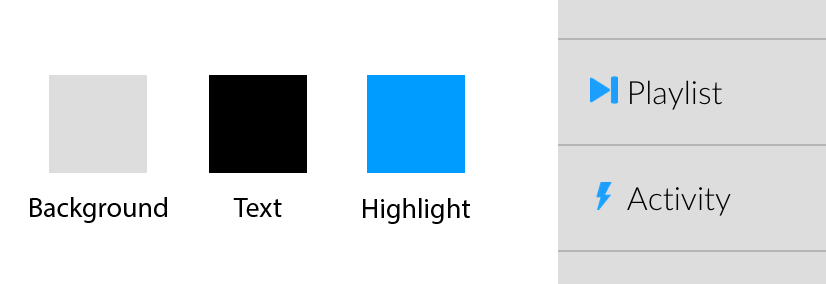
\includegraphics[width=0.8\textwidth]{./img/greybluecolours.png}
        \caption{Light grey, black and light blue}
        \label{fig:bluegrey}
\end{figure}

The second colour scheme sways more towards a dark UI. The background would be a dark grey (\#191919)  with white (\#FFF) for text and orange (\#FE6718) to highlight elements. This would fit into the dark UI scheme as talked about earlier but also because the orange signifies a community feeling. This is perfect for the concept of choona as one of its aims is to bring people together with the power of music. \\

\begin{figure}[h!]
\centering
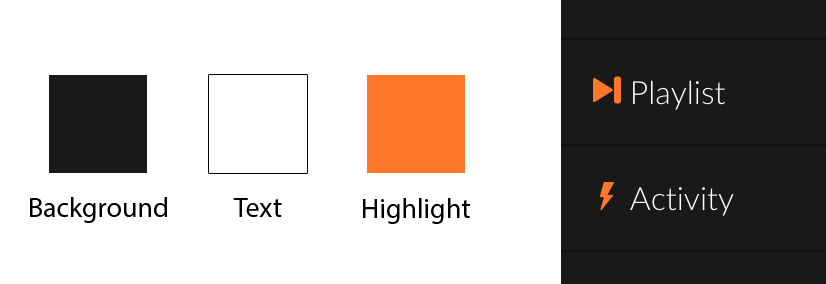
\includegraphics[width=0.8\textwidth]{./img/greyorangecolours.png}
\caption{Dark grey, white and orange}
\label{fig:orangegrey}
\end{figure}

The orange fits in better as a highlighting colour as it is quite a bright colour. Bright colours should not be over used because then they would become a distraction and cause problems in terms of readability.  \\

\noindent\underline{Choona Logo}\newline
The logo for any business is used as a method to not only identify the business but also set it apart from others. The name `Choona' is a play on the word `Choon' which is slang to describe a song or a `Tune', it also sounds like `Tuna' thus we thought the logo should be a fish. As the look and feel of the app is quite minimal, the logo should be quite minimal too. However we did not want our logo to just be a fish, looking at how a usual WiFi signal logo is designed, we thought that would be the perfect tail for the fish as WiFi represents a network of people much like Choona does. After a very simple fish being drawn, a WiFi tail was added and the image was rotated to look up, then the image was coloured to better go with the global colour scheme picked for the app. The tail will be animated in the app. This is shown in figure \ref{fig:logo}.

\begin{figure}[h!]
\centering

\includegraphics[width=0.5\textwidth]{./img/logothinking.png}
\caption{Thoughts behind the Choona logo}
\label{fig:logo}
\end{figure}


\noindent\underline{Font}\newline
There are a number of different fonts that can be considered for the application. There was a section already covered in the literature review regarding fonts. The font to be used should be clean and work well with the background and the theme of the application. Text needs to be sized appropriately so its not too big to take screen real estate but big enough for the users to read.

The first consideration is a font called BONVENOCF shown in figure \ref{fig:Bonvenocf}. This font consists of a clean font face ideal for minimal design. It's not the conventional type of font, there are some characters which possess a more rounded feel than the usual fonts. It's uniqueness will be fitting for the app; a unique looking font for a unique app. 

\begin{figure}[h!]
\centering

\includegraphics[width=0.55\textwidth]{./img/bonvenocf.png}
\caption{Bonvenocf font\footcite{bonvenocf}}
\label{fig:Bonvenocf}
\end{figure}

Next, Google's Lato font is another option shown in figure \ref{fig:lato}. This font is used globally; with Google handling over 3 billion serves every week through their font API\footcite{googlelato}. This shows that users are very familiar to this font and just by looking at the statistics its wide usage indicates the easy readability of the font.

\begin{figure}[h!]
\centering
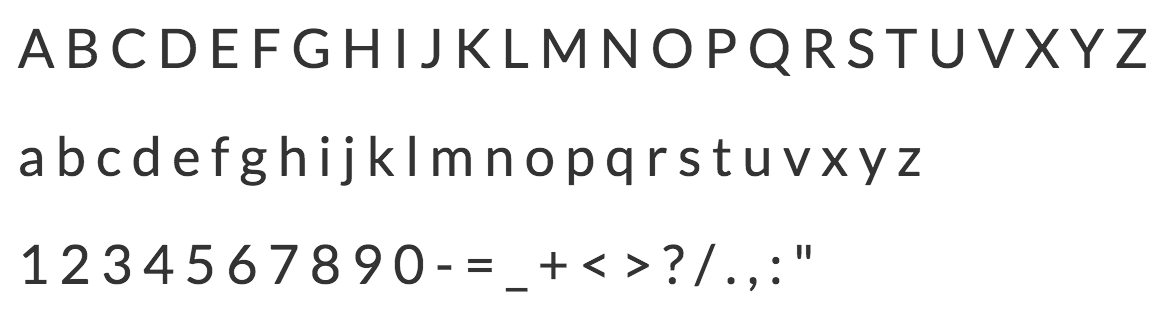
\includegraphics[width=0.65\textwidth]{./img/lato.png}
\caption{Lato font\footcite{googlelato}}
\label{fig:lato}
\end{figure}

Out of the two fonts, we believe Lato is the better fit for the application, with its clean minimal approach fitting in perfectly with the choona ecosystem.  The statistics speak for themselves; there is a clear reason this font is widely used.\\

\subsubsection*{UI Mock-ups}

The different pages of the app will be looked at closely, discussing different elements of the page in question and the reasoning behind any design decisions taken. This section will also make clear the general overall aesthetics that choona has employed to make the user's life much easier while maintaining a sleek clean look.\\

\clearpage

\noindent\underline{Welcome pages}\newline

The welcome pages will be shown to the user when they first install the app so they can quickly familiarise themselves with what it is about. Here information should be very clear and very simple as this is the first thing the user will see; they do not want to be overloaded with information. \\

\noindent
\begin{figure}[h!]
\centering
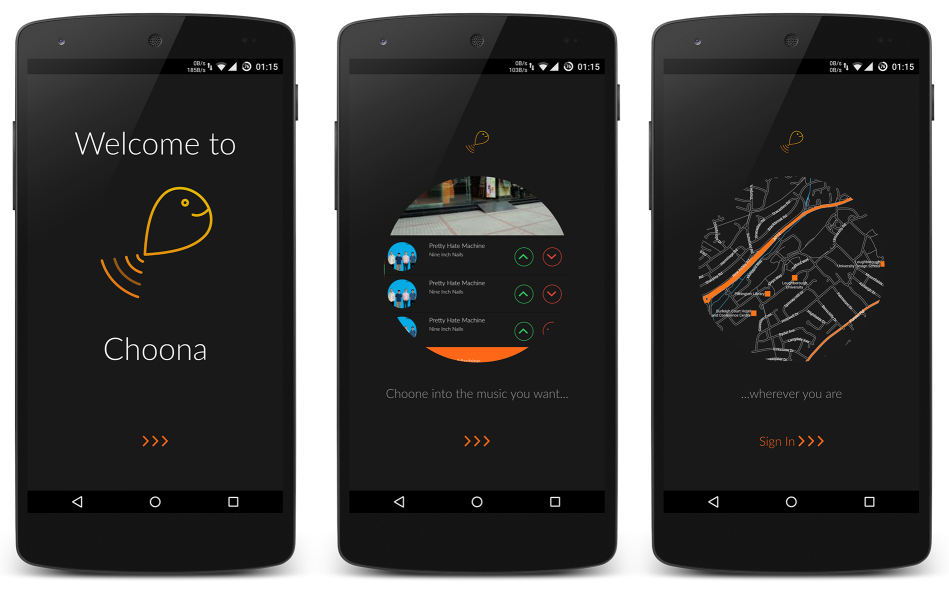
\includegraphics[width=0.95\textwidth]{./img/welcomeframed.png}
\caption{Welcome screens}
\label{fig:welcomescreens}
\end{figure}

Here the idea is to use multiple `slides' that the user can swipe through to reach the welcome screens. As shown in figure \ref{fig:welcomescreens} the users are first greeted with the Choona logo and a welcome message before moving onto two screens that describe what Choona does in one phrase; `Choon into the music you want....wherever you are'. These screens are split as this gives the chance to display the playlist page and a geolocation map, showing that Choona can be used anywhere. The user can then slide to the next page where they are asked to sign in. 

The concept clearly follows the rules here with each slide having minimal information but still making it clear on what the application is about. The use of a multi-step welcome screen here not only gives a dimension of interactiveness to the user when starting the app but it also lets the app know that the information on the page swiped has been acknowledged by the user.  

\clearpage

\noindent\underline{Login page}\newline

\noindent
\begin{figure}[h!]
\centering
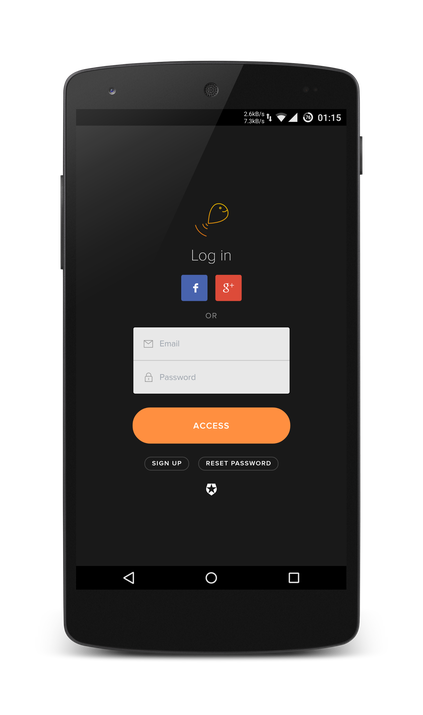
\includegraphics[width=0.45\textwidth]{./img/loginframed.png}
\caption{Login screen}
\label{fig:loginscreen}
\end{figure}

For the login page will be using auth0 authentication.  There is a template provided by auth0 to implement for these purposes. This template can be changed if needed and themed to the developers liking.  We have kept it very simple with small changes to the background and the addition of a logo.

This screen already takes care of the clean look that Choona is aiming for, the form is laid out very well with all the buttons arranged so that the user is not confused. A clear distinction is made between logging on via a social network or through an email address (both need to be available). The sign-in button is clear and well placed and makes use of the Choona orange which ties up our theme.\\

\clearpage

\noindent\underline{Side menu page}\newline

\noindent
\begin{figure}[h!]
\centering
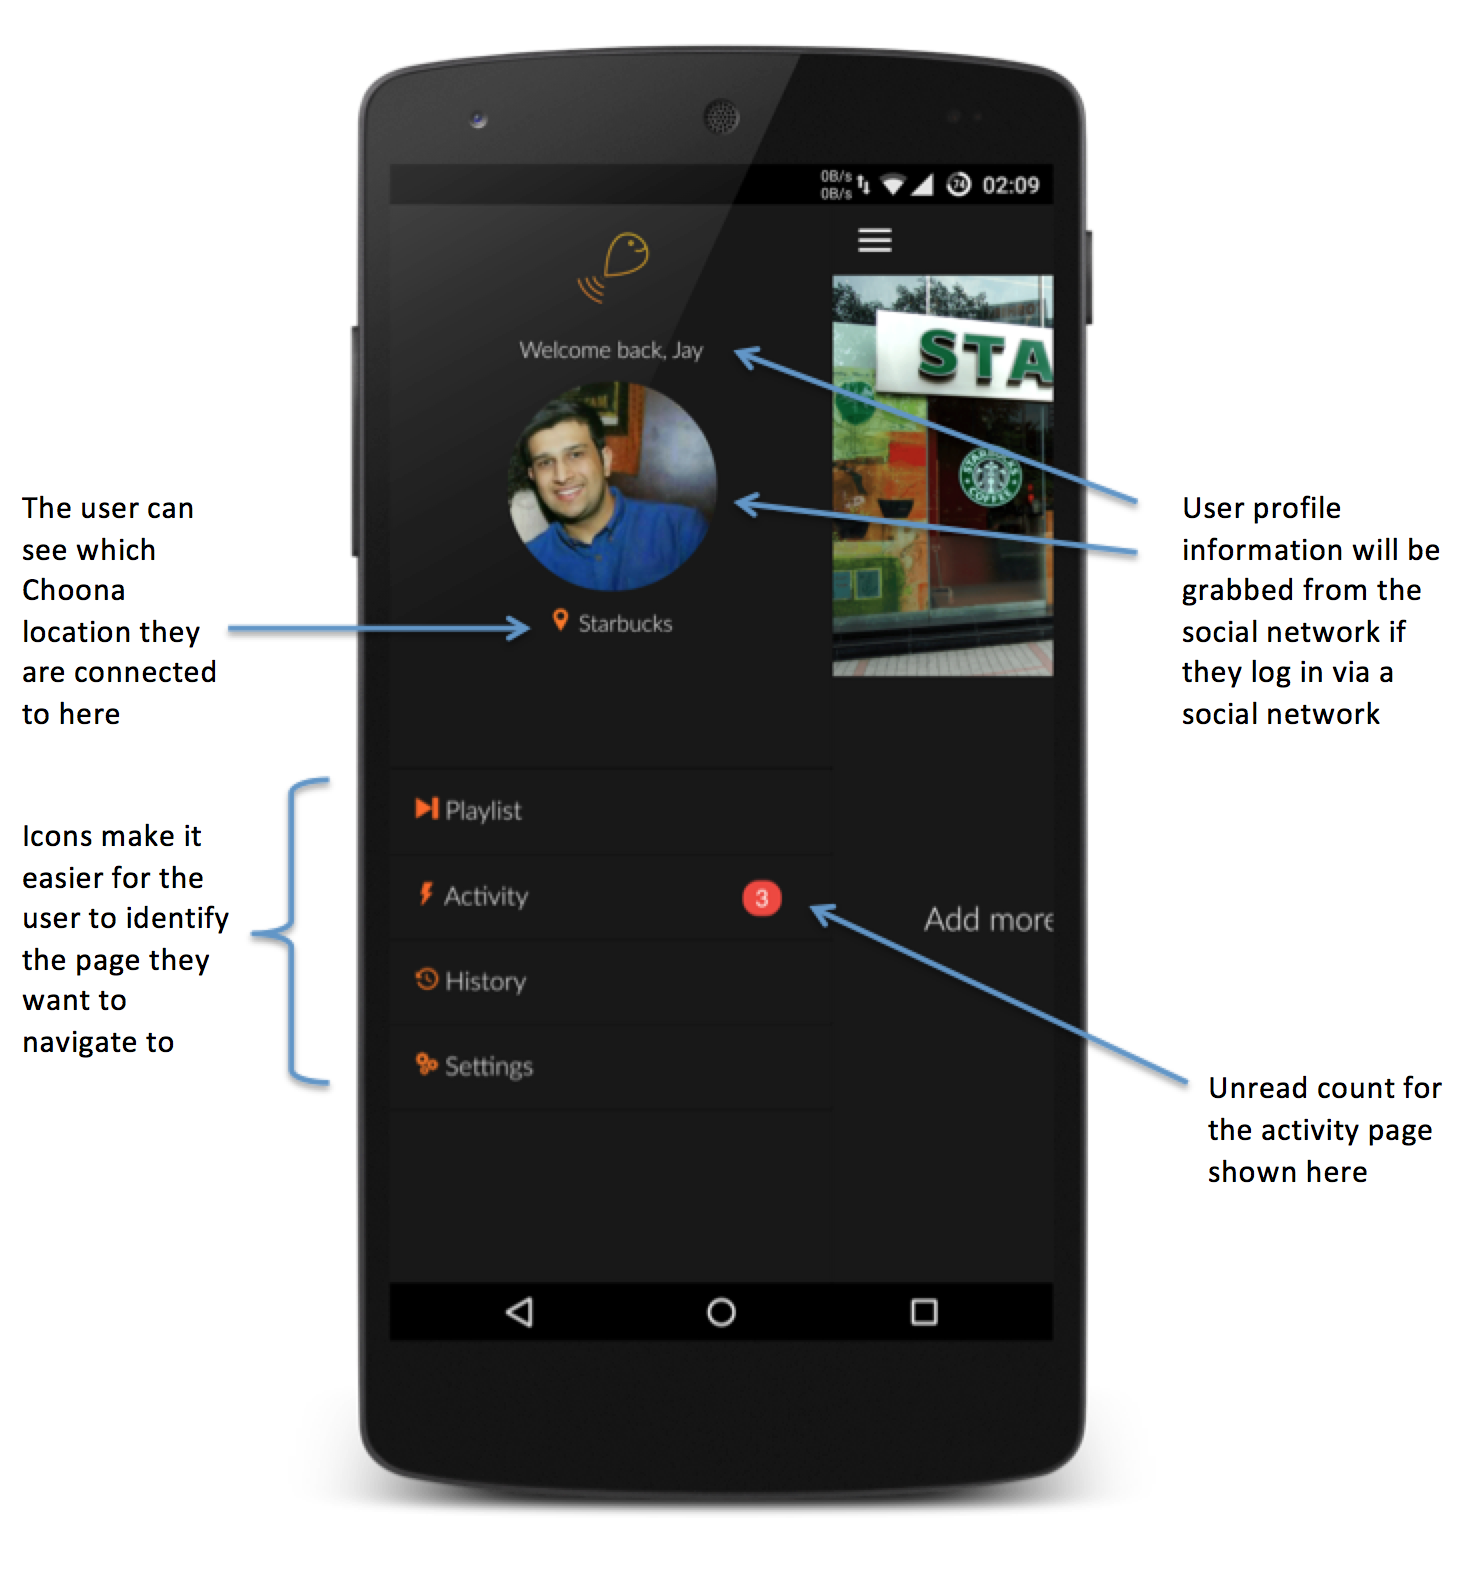
\includegraphics[width=0.76\textwidth]{./img/sidemenuannotated.png}
\caption{Side menu page}
\label{fig:sidemenu}
\end{figure}

The side menu page will be used by the user to navigate the app. It's important that this page is simple and straight forward or the user will not be able to find what they need or do what they want. The profile section positioned at the top assures the user they are logged in and welcomes them to Choona.  Below the profile image, the name of the Choona location they are currently connected to will be shown. Moving down the screen, all the different pages are listed. Each page has an icon, this makes it visually easy for the user to move to different pages and also to identify the pages. Additionally on the activity page, an unread count is shown in the side menu so the user knows if there are any unread activities.\\

\clearpage

\noindent\underline{Playlist page}\newline

\noindent
\begin{figure}[h!]
\centering
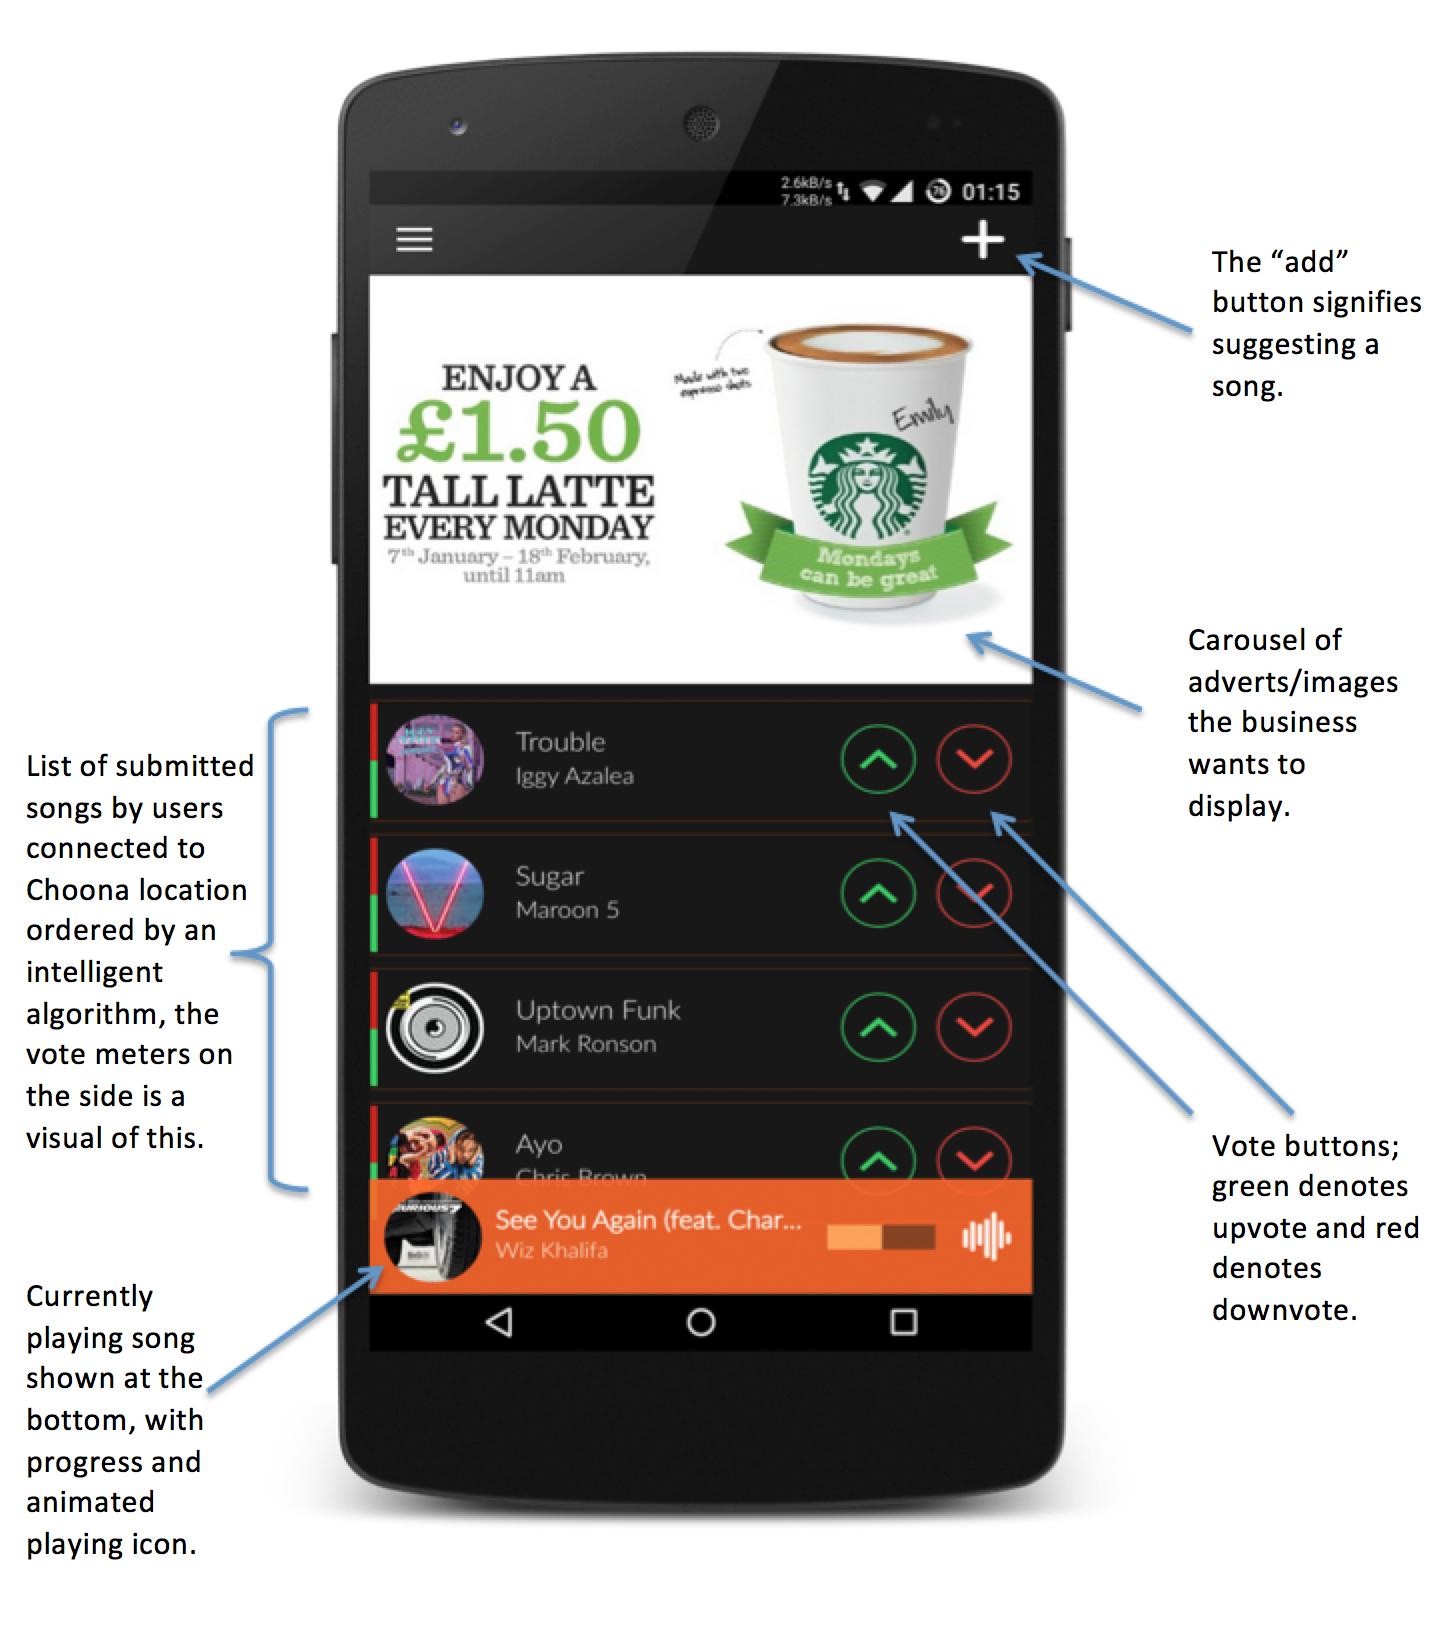
\includegraphics[width=0.65\textwidth]{./img/playlistannotated.png}
\caption{Playlist page}
\label{fig:playlist}
\end{figure}

This is one of the most important pages in the application, here the user will be able to vote on the songs suggested and also have access to the search page where they will be able to add a song. From the top, the user will see a carousel of images which the business will set up beforehand, this could be adverts for the business. Below there will be the list of suggested songs by others. These are in a list with each song containing an up-vote and down-vote button.  Everything is spaced evenly so the user can scroll and vote with ease. The user is also presented with a live vote-meter on the left of every song item in the list. This adds another dimension to the app where they can visually see how well that track is doing (more votes = higher up the list); denoted by appropriate green and red bars in the `votemeter'. Finally at the bottom, the now playing bar shows the current song being played. This bar can be tapped on to access the now playing page; this is conventional in most music applications, such as Google play music.

\clearpage


\noindent\underline{Search page}\newline

\noindent
\begin{figure}[h!]
\centering
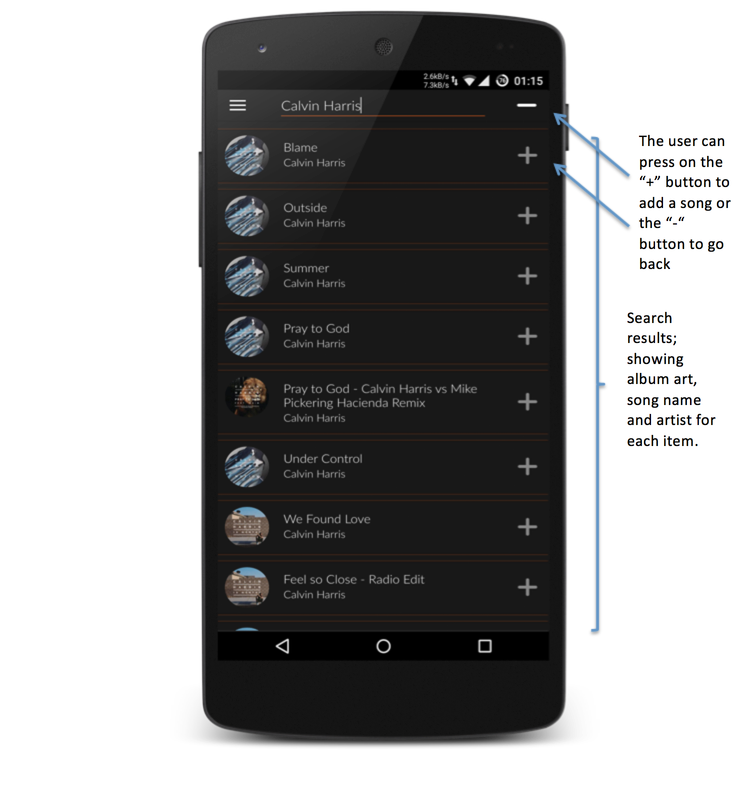
\includegraphics[width=0.7\textwidth]{./img/searchannotated.png}
\caption{Search page}
\label{fig:searchpage}
\end{figure}

Through this page, the user will add a song, thus it is important that this screen is easy to follow. When the user starts typing all the results will be shown as indicated in figure \ref{fig:searchpage}. Beside each song, a `+' sign will appear, similar to the one on the playlist page signifying they want to add that song to the playlist. The `-' button can be used to got back and cancel the search. 

This is a very simple approach to the search page and by only showing the vital information, the user does not get overloaded with information. An alternative solution here would be to display fuller album covers but this would mean more space will be taken per item which would make it harder for users to scroll through all the search results. Thus this solution would be friendlier to smaller screen devices.

\clearpage

\noindent\underline{Now playing page}\newline

\noindent
\begin{figure}[h!]
\centering
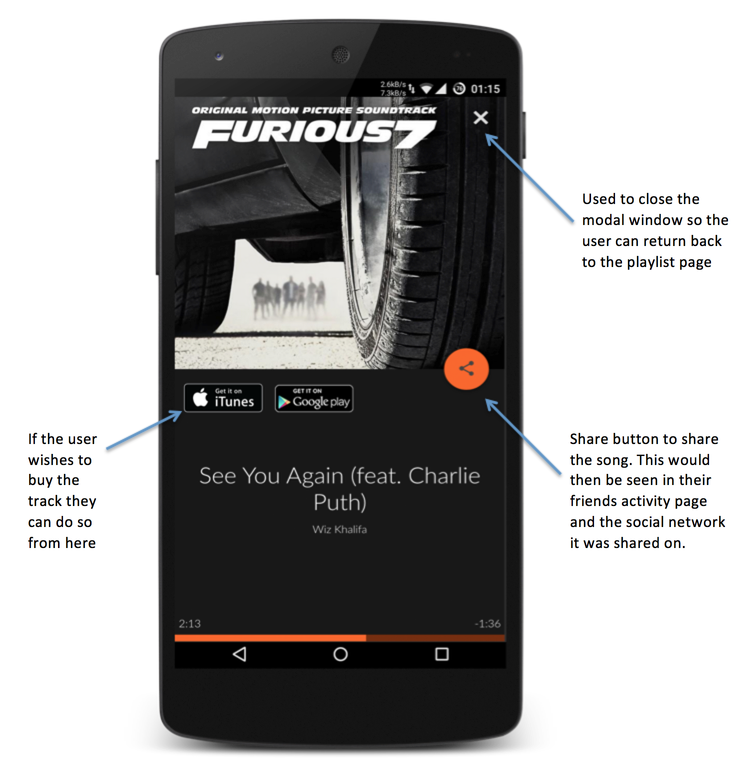
\includegraphics[width=0.8\textwidth]{./img/nowplayingannotated.png}
\caption{Now playing page}
\label{fig:nowplaying}
\end{figure}

The aim of this page is to show clear artwork and song information to the user. Furthermore there will be links to buy the song (one of the revenue streams for Choona) and also to share what they are listening to and where. The share button will be placed as a floating button much like the android lollipop ecosystem. Taking all this mind, a very minimal approach for the screen is taken here, spreading the information across the page and making use of the screen real estate. There is also a track scrubber at the bottom of the page, not responsive to the users touch as the business is in control of the music, it is only there to let the user know how far the song has progressed.   

\clearpage

\noindent\underline{Activity page}\newline

\noindent
\begin{figure}[h!]
\centering
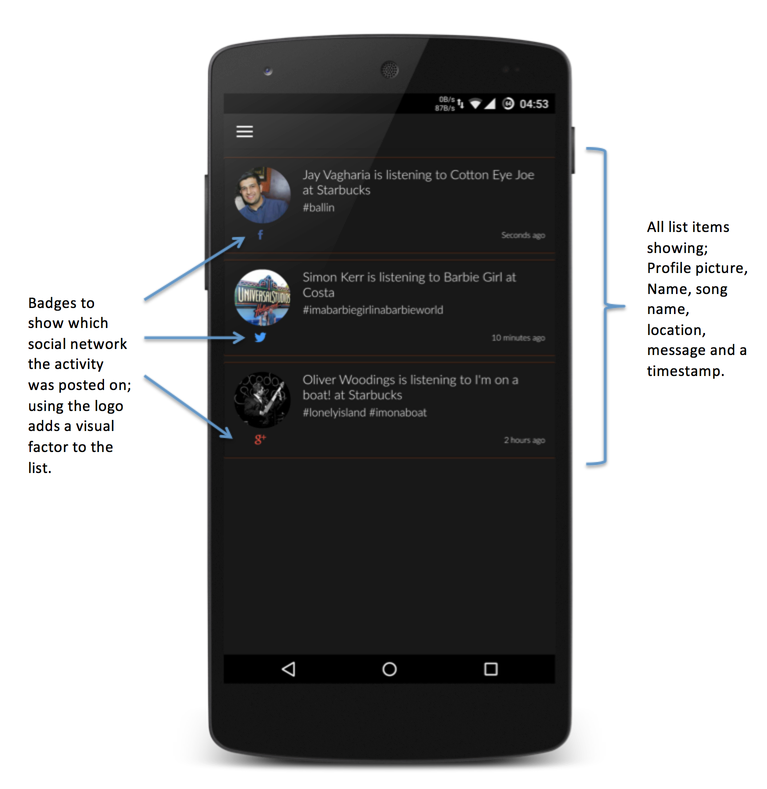
\includegraphics[width=0.8\textwidth]{./img/activityannotated.png}
\caption{Activity page}
\label{fig:activitypage}
\end{figure}

Here is all the Choona activity of the users friends will be shown. This is represented as a clear feed of items containing information to identify their friend the song and their location. An activity item will be placed on this page when the user's friend decides to use the share button on the now playing page which will fire the event. The activity will also be shared on the social network the user sent it to; letting the businesses promote themselves. 

The page follows the global colour scheme and also lays out all the information similar to the list of songs on the playlist page, the use of social badges makes it easy for the user to identify the social network their friends activity was shared on. 
\clearpage

\noindent\underline{History page}\newline

\noindent
\begin{figure}[h!]
\centering
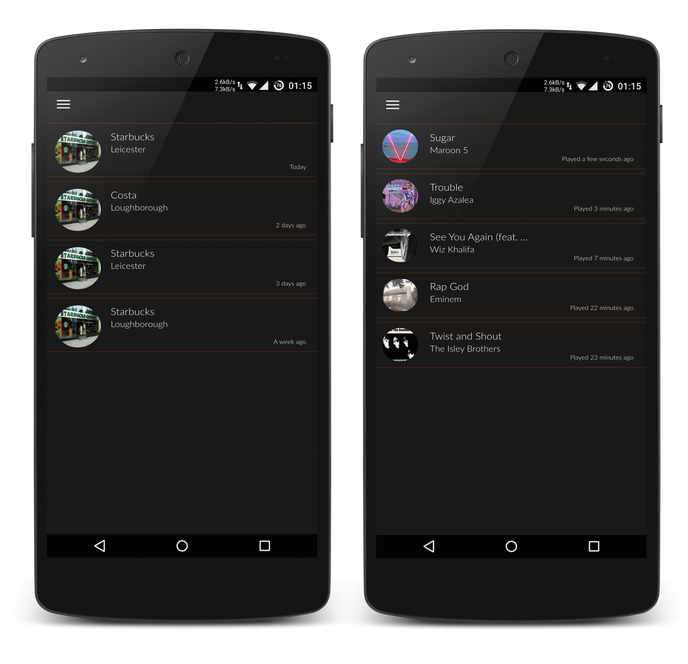
\includegraphics[width=0.77\textwidth]{./img/historyboth.png}
\caption{History pages}
\label{fig:historyboth}
\end{figure}

This page lets the user easily access any songs that were played in places they visited in the last week. First they will be shown a list of places (Left on figure \ref{fig:historyboth}) and then they can tap on a certain place to see the songs played in the time they were there (right on figure \ref{fig:historyboth}. Simple lists were used here taking the minimal approach with only showing data that the user is interested in. The styling is consistent with the other pages that employ lists in their containers.

An alternative design here would be an accordion approach where each root item would be a location and when expanded, would show all the songs played for that location for the duration that the user was there. Even though this method means that the user does not have to visit another page, it could be be very bad for scrolling through a long list of items. This would be unpopular with smaller screen phones as they will have to scroll through a lot more to find what they want.

\clearpage

\noindent\underline{Settings page}\newline

\noindent
\begin{figure}[h!]
\centering
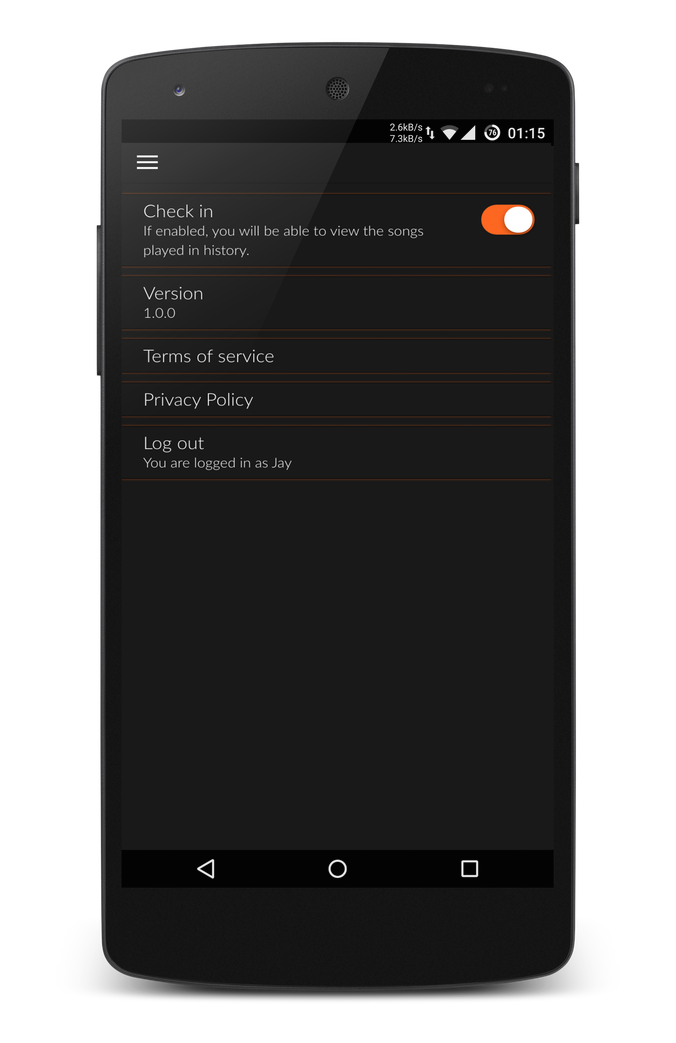
\includegraphics[width=0.55\textwidth]{./img/settingsframed.png}
\caption{Settings page}
\label{fig:settingspage}
\end{figure}

This is where the user will be able to configure the app and any options around it. At this point there are minimal things to configure on the app. One option is to toggle auto logging of history which is on by default but the user can turn it off if they wish. This is a slider button familiar to both android and iOS devices for toggling something. The log out button will also belong here in the case they want to log in with another account. 

This is another simple screen on the phone, so a minimal approach has been taken to design it. Other than the options talked about above, important information such as Choona's terms of service and privacy policy are also included in this screen.
  \clearpage
  \section{Implementation}
The system architecture proposed during the design stages has been divided into three distinct sections for development; services, API and UI. Figure \ref{fig:architecture-changes} shows how the original architecture has been adapted for the development of the prototype.

\begin{figure}[h!]
  \centering
  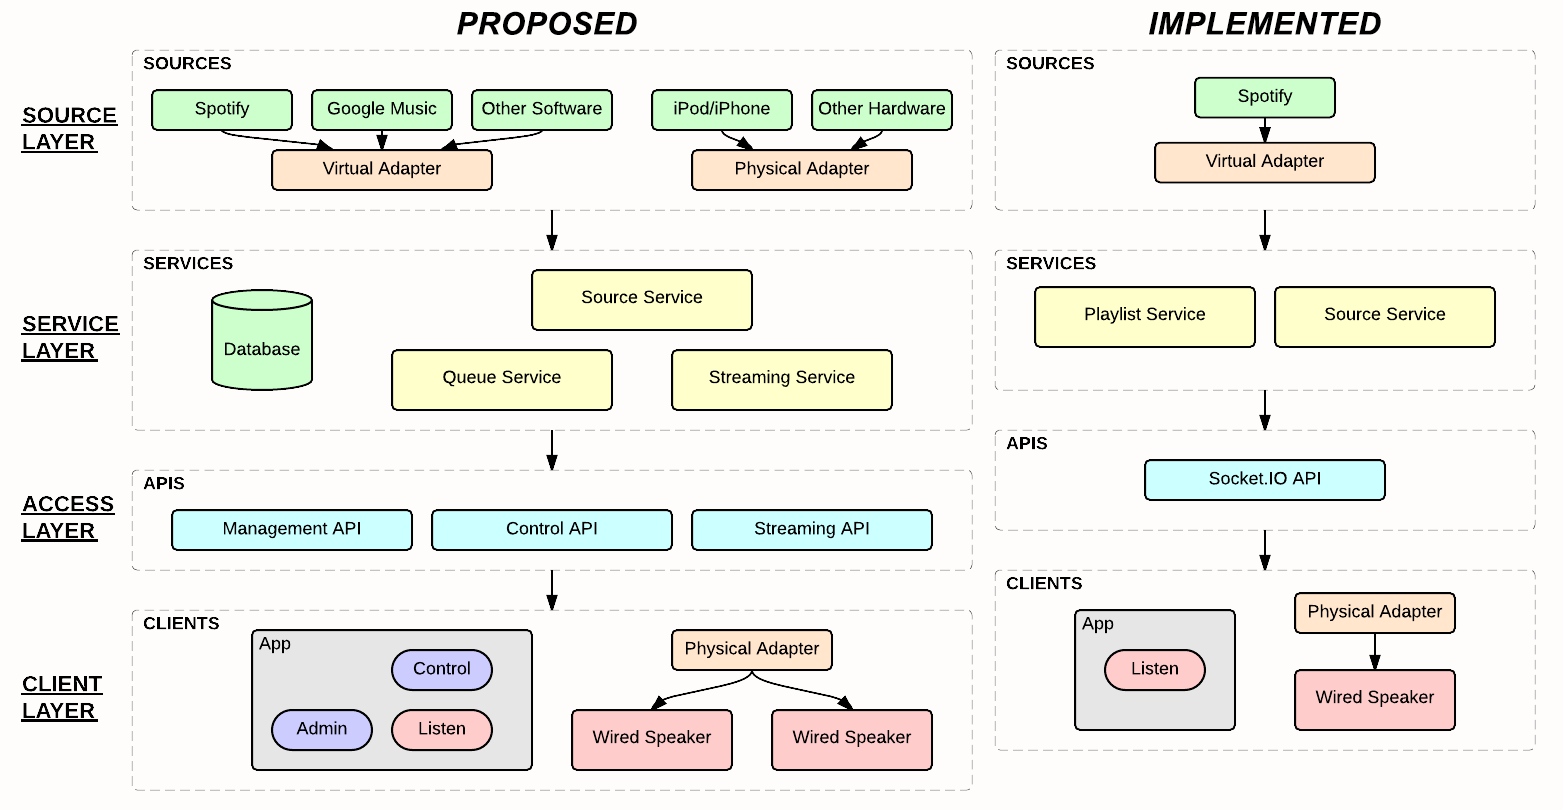
\includegraphics[width=1.02\textwidth]{./img/architecture-changes.png}
  \caption{Prototype architecture alongside original proposed architecture}
  \label{fig:architecture-changes}
\end{figure}

Spotify has been chosen for use as the first type of audio source due to it's well documented and accessible API, along with it's popularity as a personal music service. No physical audio sources, such as iPods, will be available in the prototype due to the added complexity of interfacing with a physical device.

The queue and streaming services have been joined together to create a single playlist service. This is because the contexts of the two services are very similar and can be regarded as tightly-coupled in functionality; the micro-services architecture specifies\footcite{microservicesio} that services should be de-coupled in order to promote scaling and flexibility.

All three types of APIs have been implemented as one singular Socket.IO API for the purposes of the prototype in an effort to make authentication simpler.

Finally, the management and control part of the mobile app has not been implemented due to time constraints; users will only be able to add songs, upvote/downvote tracks and listen to audio.

\clearpage
\subsection{Inter-Service Communication}

As discussed during the design stages, the micro services architecture offers many advantages over traditional monolothic software. By having everything in the system running as a service it is possible to scale the application in every direction with relative ease. It does, however, introduce the complex problem of inter-service communication. Early implementations of the architecture made use of HTTP APIs\footcite{microservices-mueller} which work well in simple applications. Relying on HTTP, however, can be seen as a restriction since it is a one-to-one client-to-server connection. In large scale applications it is often necessary to have one-to-many messaging between many different services. HTTP also requires each service to know how to connect to all other services it wants to communicate with, as shown in figure \ref{fig:http-communication}.

\begin{figure}[h!]
  \centering
  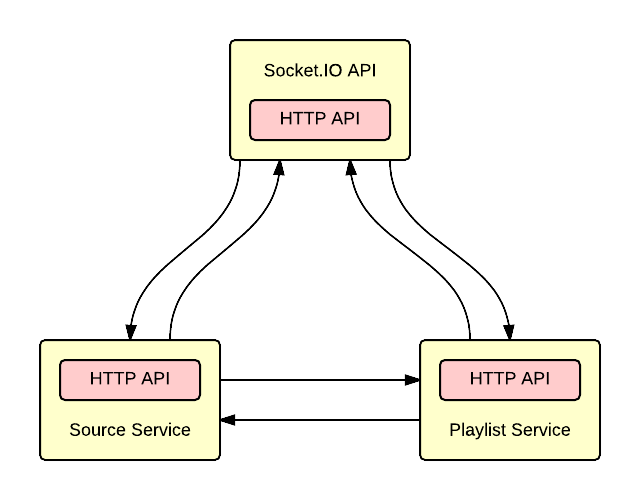
\includegraphics[width=0.6\textwidth]{./img/http.png}
  \caption{Inter-service communication using HTTP APIs}
  \label{fig:http-communication}
\end{figure}

The most popular alternative to HTTP APIs for inter-service communication is a message broker, such as RabbitMQ\footcite{rabbitmq} or Redis\footcite{redis}. In this kind of system, all nodes connect a central broker that is responsible for distributing messages. This has the advantage of a node only needing to know the location of the broker, rather than all other nodes. It also means that messages can be distributed to multiple nodes, removing the one-to-one restriction found in an HTTP-based communcation system. Figure \ref{fig:redis-communication} shows how a redis-based communcation system can be composed.

\begin{figure}[h!]
  \centering
  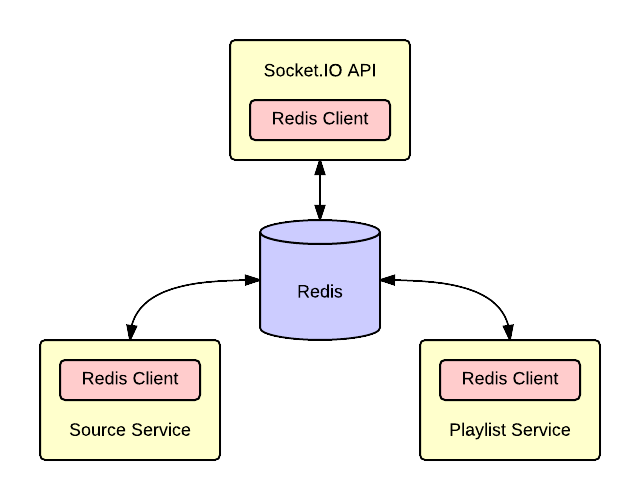
\includegraphics[width=0.6\textwidth]{./img/redis.png}
  \caption{Inter-service communication using Redis}
  \label{fig:redis-communication}
\end{figure}

Messaging systems solve the problem of distributed inter-service communication, however they do introduce their own restrictions. Messages are very low-level; they are simply a single piece of data being transferred between two points. They are entirely stateless and do not support any kind of meta data. It is therefore necessary to treat a service like Redis as a transport and implement a higher-level protocol on top.

This has been achieved in Choona by creating a new communication library called Waterway\footcite{waterway}, built on top of Redis. The roles for both Waterway and Redis can be defined as follows:

\textbf{Waterway:}
\begin{itemize}
  \item Expose an API for three types of high-level messages:
    \begin{itemize}
      \item Streams: a continuous flow of individual messages (such as audio data)
      \item Requests: a single message with a guaranteed response (synonymous to an HTTP request)
      \item Events: a single message with no response (such as a status report)
    \end{itemize}
  \item Translate between high-level messages and low-level redis messages, identified with keys
\end{itemize}

\textbf{Redis:}
\begin{itemize}
  \item Provide an open transport for any type of data to be sent as a message
  \item Distribute messages to nodes by pattern matching the message keys
\end{itemize}

As shown by figure \ref{fig:waterway-communication}, Waterway replaces the role of the standard Redis client in a service. This is where the translation between high-level Waterway messages and low-level Redis messages occurs.

\begin{figure}[h!]
  \centering
  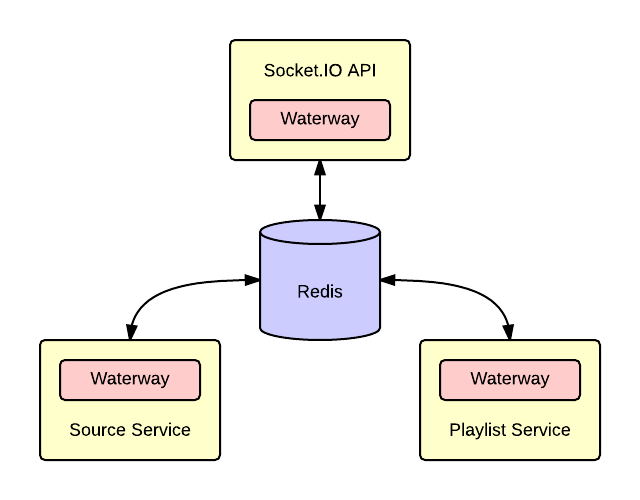
\includegraphics[width=0.6\textwidth]{./img/waterway.png}
  \caption{Inter-service communication using Waterway}
  \label{fig:waterway-communication}
\end{figure}


\subsection{Audio Streaming}

Choona allows multiple clients to connect and listen to the same audio stream. This means that each client needs to be listening to the same audio at the same time, otherwise the whole system will become out of sync. The easiest way to achieve this is to always ensure the audio is being broadcast live, with a very small buffer window (in the same way that when watching television you always see what everone else does). Waterway makes this process relatively simple due to it's support of streams. As soon as the audio data is received from an audio source such as Spotify it is buffered and streamed out to other services at the exact bitrate of the song. This ensures that all services in Choona see the exact same audio data and the exact same time. It also has the added advantage of allowing the playlist service to know precisely when a track starts and stops; it can just wait for the buffered audio stream to end. Choona's streaming pipeline is described in figure \ref{fig:streaming}.

\begin{figure}[h!]
  \centering
  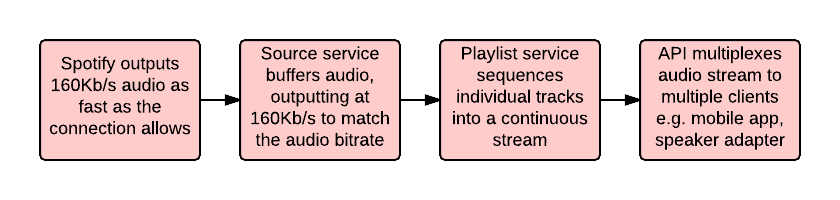
\includegraphics[width=1\textwidth]{./img/streaming.png}
  \caption{Buffered audio streaming through the Choona audio pipeline}
  \label{fig:streaming}
\end{figure}

Clients can then choose to handle the audio in whatever method they prefer; for example, in a browser-based environment the MP3 stream can be converted into raw PCM audio data and played out of the device using the HTML5 Audio API.


\subsection{API}

Socket.IO is a realtime bi-directional communcation protocol and library, designed to replace standard HTTP-based web communcation. For Choona, Socket.IO offers the following benefits:

\begin{itemize}
  \item \textbf{Bi-directional communication:} HTTP is a client -> server model, where only the client can initiate requests. This is fine for regular websites, however it does not work for scenarios where the server needs to send requests without the client initiating them, such as a realtime application like Choona. To counter this there are now several different strategies and protocols for handling bi-directional communcation on the web, many of which are supported by Socket.IO such as WebSockets and long polling.
  \item \textbf{Device support:} Socket.IO will select the best available bi-directional protocol supported by both the client and server when setting up connections, resulting in almost all devices being supported.
  \item \textbf{Binary data support:} As specified in the requirements, the Choona app will need to be able to play audio out of the phone speakers/headphones. This means the audio data will need to be streamed into the app. Socket.IO has built-in support for correctly transferring binary data which means the audio can be streamed using the same communication and authentication methods as the rest of the app.
\end{itemize}

Choona's Socket.IO API acts as a simple gateway between clients (such as the mobile app) and the many services that make up the backend infrastructure. It has three main objectives:

\begin{itemize}
  \item authenticate users
  \item ensure requests are authorised
  \item proxy requests to other services in the system
\end{itemize}

The API can almost be interpreted as a firewall; it protects the internal services from being unauthorised access and ensures users are authenticated. It also means that clients do not and cannot know about the internal structure of Choona's architecture which adds an element of security by secrecy.


\subsection{Authentication}

Choona's user authentication is managed by the SaaS platform Auth0. It is now commonplace for applications to allow users to authenticate with many different third parties such as Facebook and Twitter. Developing and maintaining support for even one type of authentication can often prove to be fairly involved, let alone 3 or 4. Auth0 helps developers with this problem by abstracting all the different authentication providers into a single API, giving many advantages\footcite{auth0}:

\begin{itemize}
  \item Only need to implement one authentication system
  \item Quickly build embedded login forms using the Auth0 libraries
  \item Manage all users from a central management interface (Figure \ref{fig:auth0-users})
  \item Easily maintain a single, common view of the user's data
  \item Integrate with existing user databases
\end{itemize}

\begin{figure}[h!]
  \centering
  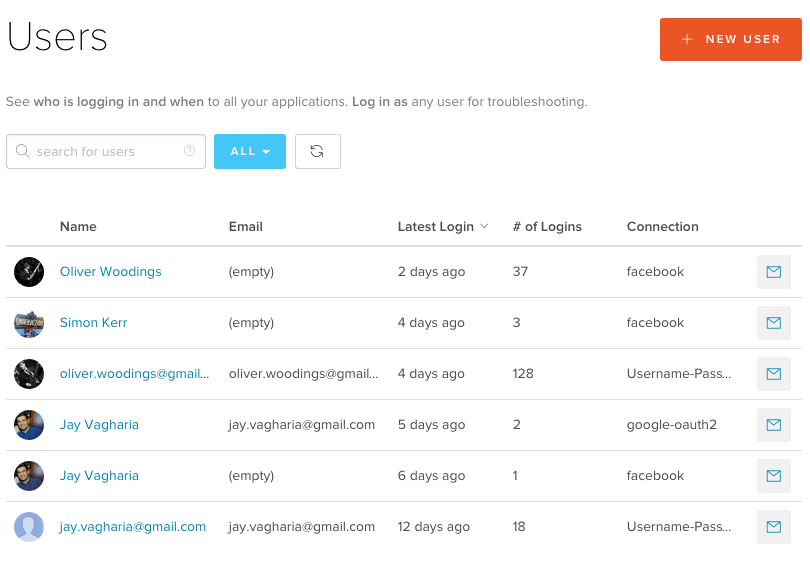
\includegraphics[width=0.6\textwidth]{./img/auth0-users.png}
  \caption{Auth0 user management}
  \label{fig:auth0-users}
\end{figure}

Auth0 handles the entire login and authentication process without needing any changes to an application's server-side systems. This is achieved by using JSON Web Tokens; a unified way of structuring and encoding authentication data into a JSON object. This object is then encrypted using a private key, allowing it's integrity to be easily validated by third parties using the corresponding public key. JSON Web Tokens are used by the Choona API to ensure a user is authenticated and also to extract information about them for use in other services. This process is shown in figure \ref{fig:auth-process}.

\begin{figure}[h!]
  \centering
  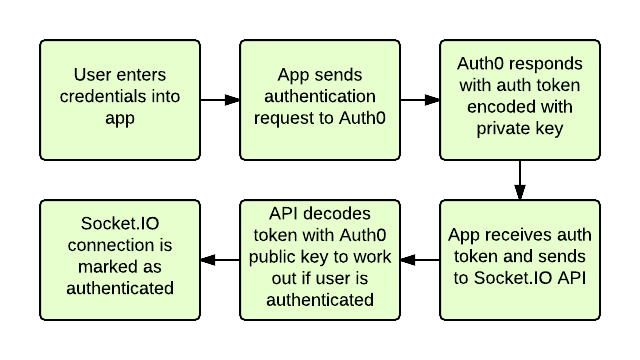
\includegraphics[width=0.7\textwidth]{./img/auth-process.png}
  \caption{Choona authentication process}
  \label{fig:auth-process}
\end{figure}


\subsection{Speaker Adapter}

As part of this first iteration of development a prototype of a Choona speaker adapter has been made. The hardware used is a Raspberry Pi 2 Model B running the Raspbian operating system. The software itself is designed to be as autonomous as possible; once the device has an internet connection it will automatically connect to the Choona API, authenticate and start streaming to music from the pre-configured playlist. This is then outputted from the jack socket of the Raspberry Pi into whatever speakers or headphones are connected.


\subsection{UI}

The Choona mobile app is made using the Ionic framework, which itself is built on top of AngularJS. As discussed in the design stages, building a mobile app using web-based technology allows it to easily be deployed to any platform. Ionic makes this even easier by making available a set of mobile-friendly UI components\footcite{ionic}. Figure \ref{fig:phonegap} shows how PhoneGap/Cordova is used to take the Choona sourcecode and compile it into ready-to-deploy applications for each mobile platform.

The app itself is structured like a typical AngularJS application, using factories, states, controllers, scopes and views:

\begin{itemize}
  \item \textbf{Factory:} a constructor that instantiates or prepares an object for use in the rest of the app
  \item \textbf{State:} a component of the routing state machine used to navigate around the application and render different views\footcite{router}
  \item \textbf{Controller:} responsible for interfacing between views and the rest of the app
  \item \textbf{Scope:} each controller/state has it's own scope for containing variables and methods, which is inherited and extended from parent scopes
  \item \textbf{View:} HTML mixed in with Angular's data binding syntax
\end{itemize}

\begin{figure}[h!]
  \centering
  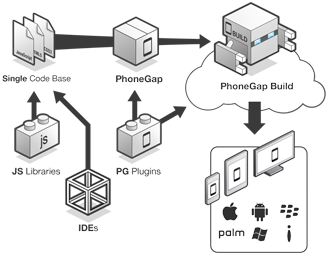
\includegraphics[width=0.5\textwidth]{./img/phonegap.png}
  \caption{PhoneGap/Cordova build process\footcite{phonegap}}
  \label{fig:phonegap}
\end{figure}

Figure \ref{fig:state} shows Choona's application state/scope tree. Children inherit the scopes of their parents, which makes it possible to pass properties and methods from the root scope all the way down to nodes at the bottom of the tree. This inheritance also makes it simple to implement authentication restrictions; by applying the restriction in the App state the application will also inherently prevent access to all the child states.

\begin{figure}[h!]
  \centering
  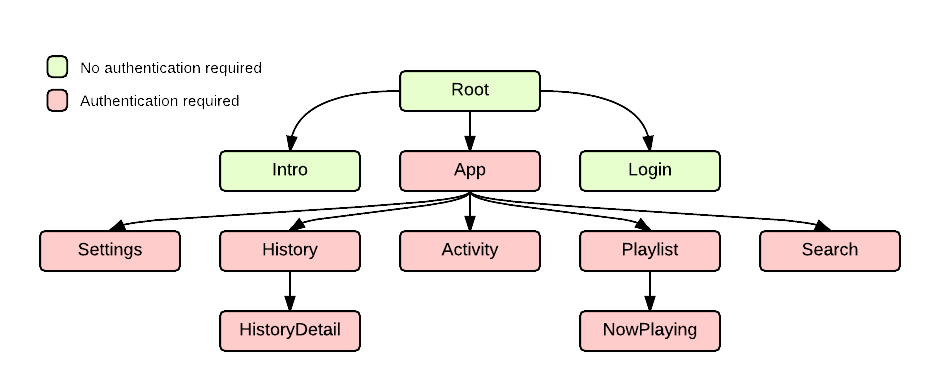
\includegraphics[width=0.9\textwidth]{./img/state.png}
  \caption{Choona's application state/scope tree}
  \label{fig:state}
\end{figure}

Scope inheritance is used in Choona to share data between controllers and views, creating a \textit{single source of truth}. This is achieved by storing application-wide data on the highest possible node in the tree; in this case it is the App state. For example, the current playlist information is stores on the App scope since it is required by both the Playlist and History states. If the data was stored on each node individually it would create two different sources of truth that would both need to be maintained separately. All data received from the Socket.IO API is stored at the application level in order to preserve this single source of truth. When data needs to be sent back to the Socket.IO API it is the responsibility of the closest controller/scope to the source of the action. For example if a user upvotes a song on the playlist, it is the role of the playlist controller to inform the API about the change. This whole process is the \textit{data lifecycle} of Choona, and is visualised in figure \ref{fig:lifecycle}.

\begin{figure}[h!]
  \centering
  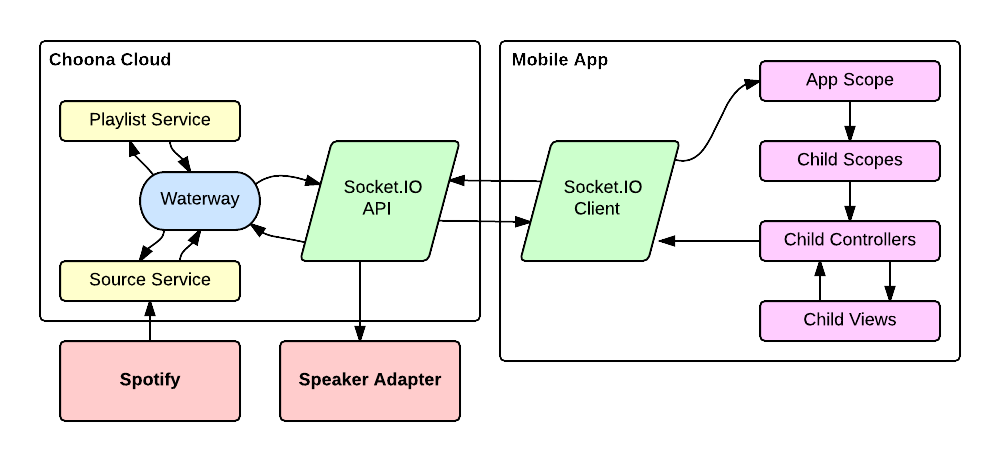
\includegraphics[width=0.9\textwidth]{./img/lifecycle.png}
  \caption{Data lifecycle of the entire Choona ecosystem}
  \label{fig:lifecycle}
\end{figure}
  \clearpage
  \section{Evaluation}

\subsection{User Feedback}
Once the prototype had been completed, we wanted to receive some user feedback on the general idea of Choona and the client side app. This feedback will help us determine whether or not the system so far satisfies its intended purpose. This testing has been carried out on a small group of participants that covered a broad customer base allowing us to gain useful feedback.

\subsubsection{Feedback conditions}
We decided to make use of our Raspberry Pi adaptor to test its capabilities when there were multiple users interacting with the system at once. The app was then placed on everyone's mobile device. After the session was over, the participants were asked to complete a survey (created using survey monkey\footcite{survey}).  

\subsubsection{Results}
There were a total of 17 participants; 10 male and 7 female. The age of these participants aired between the ages of 18 and 54. The highest number of participants were within the 18-24 category.    
From the users feedback, we noticed a level split between the two major operating systems with Android being used by 35\% of the participants and iOS used by 40\% of participants.  This correlates with our findings during the literature review.  The participants spread for mobile device operating system.  \\
The participants generally seemed interested in music as shown in figure \ref{fig:interest_music}.  53\% were interested in music with 41\% very interested in music.  \\

    \begin{figure}[h!]
      \centering
      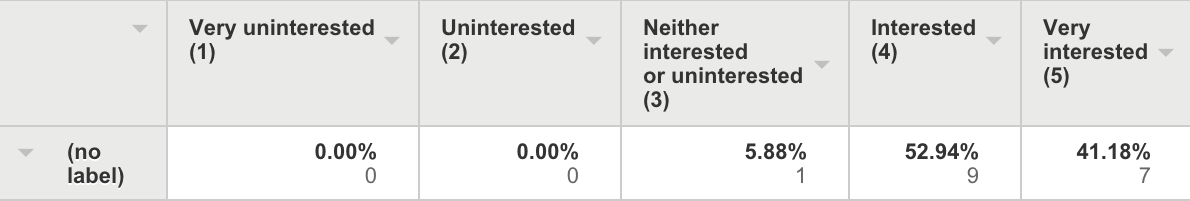
\includegraphics[width=0.8\textwidth]{./img/music_interest.png}
      \caption{Participants interest in music}
      \label{fig:interest_music}
    \end{figure}

The feedback we received for overall experience of Choona was very positive with 47\% very satisfied and 47\% satisfied with the majority of users happy with the look and feel of the app (59\%).  Navigation around the app was deemed easy (88\% of users).  \\
During our research, we discovered what makes a UI effective and we tried to incorporate this into the app.  This feedback has highlighted that we are along the right tracks and have a solid foundation.  However, with 2 individuals neither satisfied or unsatisfied with the look, feel and navigation, it shows we still have work to do.  One of the areas mentioned to us was the `up-vote/down-vote' buttons on the playlist - other ways to display this type of feature.  \\

We also asked for input on how often they would use Choona.  Just over 10\% came back and said they would use it extremely often (all the time).  Very often received 47\% of the vote and moderately often received 34\% of the vote.  These figures were slightly lower than we had hoped for.  we were hoping for a slightly higher `extremely often' response.  This identifies to us that there will be different situations when a user feels they will be in a situation to use Choona but decide they won't want to.  Although this can be the case sometimes, we want users to be using Choona as much as possible.  We want the experience to be rewarding enough for them to constantly be using it.  Therefore, this has identified an area we can improve upon; to make Choona more applicable in any situation.  \\

    \begin{figure}[h!]
      \centering
      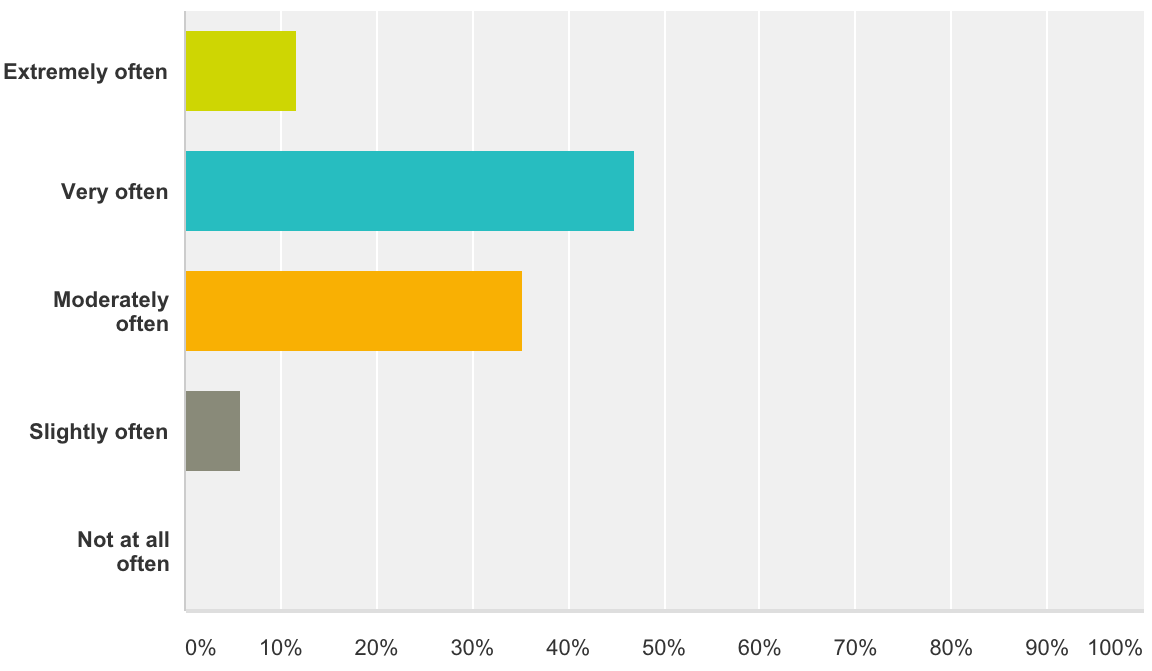
\includegraphics[width=0.8\textwidth]{./img/how_often.png}
      \caption{How often they would use Choona}
      \label{fig:how_often}
    \end{figure}

Linked to the previous question, participants were also asked when they would make use of Choona and the results are shown in figure \ref{fig:where}.  This highlights that the most popular options are coffee shops, bars/restaurants and nightclubs.  This is useful feedback as this will help us position our service in the right way to make sure we have a good initial user base.  As you can see, there wasn't an unanimous result for any one situation.  So users are telling us that they all have different preferences for the use of Choona.  This is vital information and is something that we believe we need to work on.  We want to make sure that all scenarios fit with Choona.  \\

    \begin{figure}[h!]
      \centering
      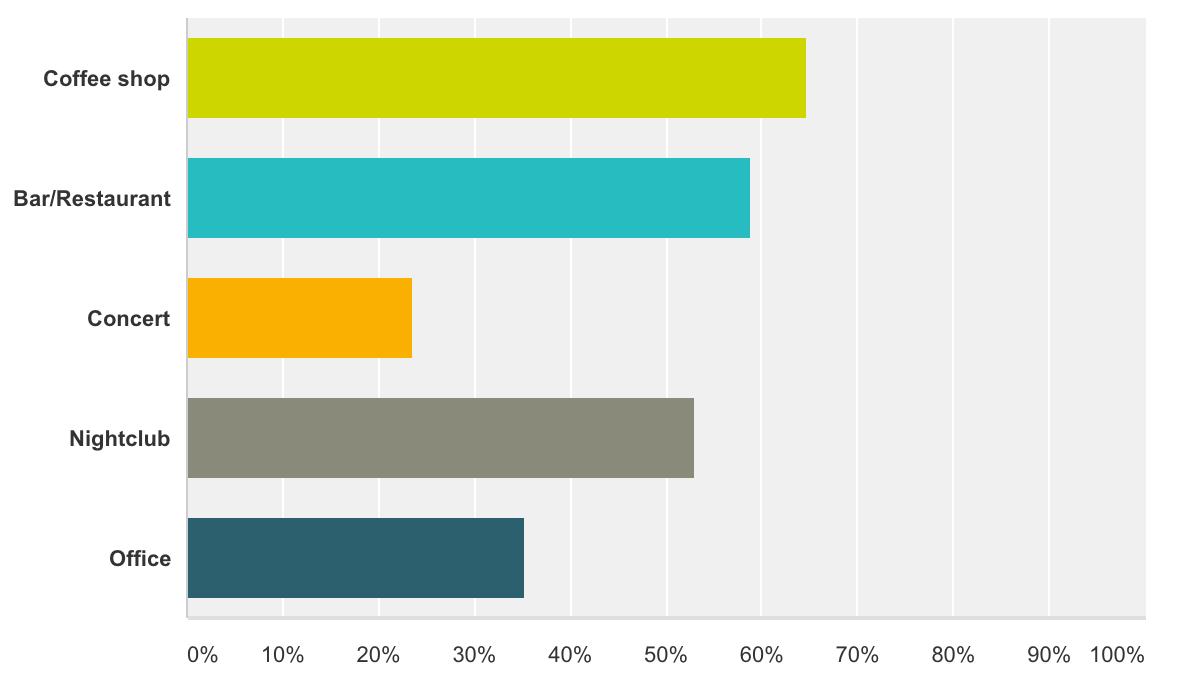
\includegraphics[width=0.8\textwidth]{./img/use_situation.png}
      \caption{Where they would use Choona}
      \label{fig:where}
    \end{figure}

The final question was whether or not the participant would recommend Choona to a friends or family.  All seventeen participants said `yes'.  This feedback signifies that we have come up with a service that actually provides value to a customer and something that is significant enough to recommend to other people.  

\subsubsection{Conclusion}
There are several different pieces of information that we can take from this feedback session.  Firstly, the overall feedback about Choona is positive; a unique idea filling a gap in the market and confirmation that the app itself is a good basis to work from.  We need to go away and make some fundamental changes; design including buttons and layout but all features within the app received positive feedback with no one indicating that a feature was redundant.  We did receive some comments that reflected additional features we could add to the app such as a `current charts' page.  This would show the most played songs over a week long period and could include a `Choona chart' where this shows the most popular songs across the entire choose network or a top chart for a particular franchise e.g. a Starbucks chart list.  The results of the recommendation of Choona question is something that will provide motivation to move further ahead with this project.

\subsection{Market Readiness}

The Choona prototype has proved that the idea itself works as a technical system and is well received by users, however there are still several important milestones to complete before Choona is be ready to release to the general public.

\begin{itemize}
  \item \textbf{Audio Licensing and Partnerships}\\
    We've previously discussed the issues surrounding music licensing for public locations and how they can be resolved, however another hurdle that will have to be tackled is the restrictions that many audio sources have in their terms of service. Spotify, for example, has a blanket ban on using their service in any commercial or non-personal environment\footcite{spotifypublic} with the exception of official partnership agreements\footcite{spotifypartners}. This is most likely going to be the case for most, if not all, online music services, meaning we will have to approach each company on a case-by-case basis with a partnership proposal. On the surface this may just seem like a business development issue, however it could also have an impact on Choona's software as well. For example, Spotify might require their own logo and advertising to be embedded in the app which will require additional development work and integration with third party systems.

    There is also a possibility that rival music services would not be happy with Choona supporting them both; it is highly unlikely that Spotify will endorse and enter a partnership agreement with a product that is also in a partnership with Google Music, especially if the product is still in the prototype stages. Therefore in order to get to get to market in a reasonable time frame it may be necessary to focus on partnering with one or two main services initially.

  \item \textbf{Client Management Interface}
    Choona currently has no management systems or interfaces for clients to manage their accounts. We plan to implement a separate mobile application and access API called Fishtank, designed purely for use by clients and not the general public. It is becoming increasingly common for large multi-context applications to break their apps down into multiple single-context apps; Facebook's release of their separate Pages Manager\footcite{facebookpages} is an excellent example. Having separate applications helps to keep code bases leaner and allows you to update more frequently with less chance of breaking other functionality.

    Fishtank will offer a wide range of management options to clients:
    \begin{itemize}
      \item \textit{Geofence manipulation}: designation of geofences at verified Choona locations
      \item \textit{User management}: ability to ban users, give them rewards etc.
      \item \textit{Playlist settings}: configure default playlists to load when the user-managed queue is empty, restrict searching to only pull from a subset of available tracks, define content restrictions on available songs (such as explicit content exclusion), select different upvote/downvote algorithms to use
      \item \textit{Playlist override}: ability to skip songs on the fly, pause the entire stream, bump a song to the top of the queue
      \item \textit{Ad/offer management}: insertion of visual adverts into various placeholders of the Choona application (e.g. playlist banner), creating and integrating audio adverts into the Choona stream, target offers and adverts to specific subsets of users (e.g. give frequent users a discount)
      \item \textit{Speaker adapter settings}: control the output volume, select different geolocations
    \end{itemize}

    Without Fishtank it will be hard to appeal to enterprise clients that will be looking for a polished, well-rounded system that is easy to set up and control.

  \item \textbf{User accounts}
    We currently do not maintain any server-side data about users. This means it is impossible to store long-term data such as listening history or user access levels. In order to make this happen a database service needs to be created that will be responsible for storing account data. This will be accessible via a dedicated user service that is responsible for combining profile data from Auth0 with context-specific data from the Choona user database, as shown in figure \ref{fig:user-service}.

    \begin{figure}[h!]
      \centering
      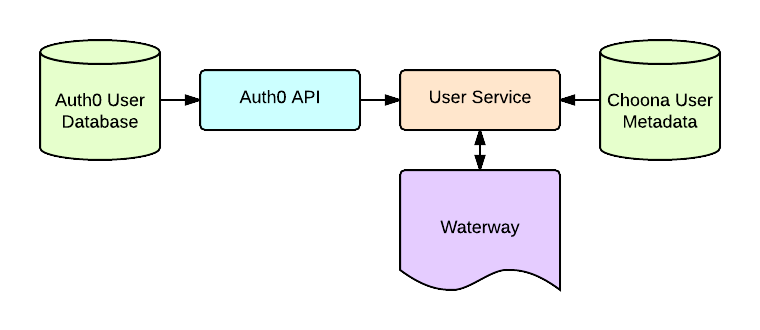
\includegraphics[width=0.8\textwidth]{./img/userservice.png}
      \caption{Future user service}
      \label{fig:user-service}
    \end{figure}

  \item \textbf{Infrastructure improvements and testing}
    The majority of the code used in the prototype is not currently covered by unit tests, making it unsafe for proper production use. Every service in the Choona infrastructure needs to have 100\% code coverage before being officially released. Furthermore every aspect of the system needs to be stress tested to ensure it is capable of supporting a high number of users. This will most likely require load balancing of certain resource-intensive services such as the Socket.IO API and the Spotify source that directly interface and manipulate audio data.
\end{itemize}
  \clearpage
  \section{Conclusion}

We believe the success of a project depends on the preparation of the individuals involved, including but not limited to:
\begin{itemize}
  	\item All members of the team playing to their strengths and identifying weaknesses
	\item Good risk management and active contingency plans
	\item Clear project requirements
	\item Always planning ahead in terms of resources, time and capacity
	\item Effective communication between the team
	\item Active communication with the client
\end{itemize}

From the very beginning of the project we all identified our particular strengths and weaknesses; as a team thought it is best in terms of resource, time and capacity management. Any weaknesses were covered by other members of the team in order to prevent an individual weakness affecting the progress of the project. Using this information, the roles were assigned to everyone and everyone knew what they were doing in the team. By the end of the project we were performing very efficiently since everyone was working on tasks assigned to their strengths. Furthermore, we had weekly meetings to ensure everyone was on track for the current milestone and to offer help to anyone that was struggling with their tasks. This did not mean that communication was restricted to the weekly meetings; if any suggestions or concerns needed to be raised we communicated through our WhatsApp group (messaging application) as we saw fit. We also had a single point of contact in the team with the client in order to prevent confusion. Any information received from the client was then distributed to the rest of the team accordingly. 

We found using Rapid Application Development throughout the project was very effective. With the frequent contact by the client, we believe we truly benefited from the short continual iterations that the development model allowed. These short iterations in development helped us to be more agile as we could quickly take the feedback from the client and adapt the solution as necessary without having to go through the entire process all over again. A good example of this workflow in practice was when we had a meeting with the client during the very early stages of the project; at that point we had a very early UI prototype to get some feedback while the backend was being developed. This meeting was very influential as he shared particular additions to the UI such as the advertisement banner on the playlist page which added another revenue channel to the application. We were able to prototype this suggestion very quickly in our next development cycle; if we were using a different less flexible development model we would not have been able to act so quickly. RAD also played well with our decision to structure the Choona ecosystem using microservices. As soon as an update was ready for a service it could be rapidly integrated, tested and deployed without having dependencies on other parts of the system.

Looking back to section 2.4, all the resources required for this project were easily accessible. The project overall was not very hardware heavy other than the raspberry pi which was provided by the department for prototyping purposes already. Due to the predominantly software-based nature of the project, version management was used to allow us to roll back changes very quickly if a RAD iteration introduced bugs. It also helped the team track different functionality additions as version increments. For this, the team used the git-based SaaS platform GitHub. The repository did not just help us have a constant backup of our work but also GitHub pushed the team to work in a more modular fashion. Features were implemented by individuals on separate branches, which were then peer reviewed by the rest of the team before being merged back into the master branch of the project. This helped keep our RAD cycles fast and bug-free and would not have been possible without the tools available in GitHub.

Reflecting more on the prototype, the chosen application frameworks used would not be appropriate if Choona was to be taken to an enterprise level. Cordova and Phonegap in general are good especially if quick prototyping is needed, however looking towards the future a more native approach might be required for better performance. This would be introduced in phases dependent upon the resources available (different developers might be needed for different mobile platforms) and the market need from the stakeholders (a need to scale the application enough where the application features demand native performance). A problem in particular was with the Ionic framework which couples with AngularJS used by the team for the prototype. Firstly the Ionic framework is very new and currently had just gotten out of beta. This raised two problems in particular; the existence of number of bugs in the framework which are still not resolved and the lack of support for the framework as its not be adapted fully just yet. Secondly the framework none of the team members had experience with AngularJS which meant the programmers in the team had to spend a long time familiarising themselves then afterwards yielding unsatisfying results because of the first issue. If we were to look back, we would not choose angularJS as a framework for the application, replacing this would most likely be ReactJS, this has a steep learning curve but is a better solution for getting the app to an enterprise level in terms of scalability. Oliver; the lead programmer in the team already has experience with ReactJS meaning we would have had a running start in terms of developing the prototype. This would mean the test of the team would have to learn React but over the long run it would have been more appropriate for the project anyways.

In relation to the risk assessment carried out, there was not any triggers that were active over the project duration, there was time over the development phase where the app would sometimes lose functionality because of a conflicting change however because we used GitHub to manage our code. This was not a problem and it was easily fixed by reverting the app back to its last working state. Secondly there were times where the app prototype would crash and lose its playlist data (this occurred in the demo) however because of the microservices architecture, the app seamlessly restarted the appropriate services without any action being taken by us. There was a loss of data here (the songs that the user suggested) but if we had more development time then songs would have been stored in persistent storage instead of memory like the prototype did, this would mean that the app would not only seamlessly recover itself by restarting any crashed services but also recover from the loss of data too with no action needed by us.

Overall, the project was a success if the context was just building a prototype, however as discussed in a number of sections there are many things that are involved in trying to get Choona to market, this involves both development elements because scalability is in question now and an added dimension to the business plan because more extensive market research needs to be carried out for it to have a valuable market presence.

  \clearpage
  \printbibliography[heading=bibintoc,title={References}]

\end{document}